\documentclass[10pt,conference]{IEEEtran} 
\IEEEoverridecommandlockouts
% The preceding line is only needed to identify funding in the first footnote. If that is unneeded, please comment it out.
%Template version as of 6/27/2024

\usepackage{tikz}
\usepackage{amsmath}

% inlined bib file
\usepackage{filecontents}
% The preceding line is only needed to identify funding in the first footnote. If that is unneeded, please comment it out.
\usepackage{cite}
\usepackage{amsmath,amssymb,amsfonts}
\usepackage{algorithmic}
\usepackage{graphicx}
\usepackage{textcomp}
\usepackage{xcolor}
\def\BibTeX{{\rm B\kern-.05em{\sc i\kern-.025em b}\kern-.08em
    T\kern-.1667em\lower.7ex\hbox{E}\kern-.125emX}}

\usepackage[all]{nowidow}
\usepackage[linesnumbered,lined,vlined,ruled,commentsnumbered,noend]{algorithm2e}
\colorlet{RED}{red}
\usepackage{listings}
\usepackage{url}

\usepackage{tcolorbox}

\usepackage{xspace}
\usepackage{multirow}
\usepackage{subfloat}
\usepackage{balance}
\usepackage{ctable}
\usepackage{listings}
\usepackage{color}
\usepackage[nobiblatex]{xurl}

\usepackage{multirow}
% \usepackage{algorithmic}

\usepackage{algpseudocode}
\usepackage{caption}
\usepackage{hyperref}

\usepackage{acronym}
\usepackage{fancybox}
\usepackage{verbatim}
\usepackage[normalem]{ulem}
\usepackage{float}
\usepackage{newfloat}
\usepackage{mdframed}
\let\labelindent\relax
\usepackage{enumitem}
\usepackage{booktabs}
\usepackage{pifont}
% \usepackage[ruled,linesnumbered]{algorithm2e}

\usepackage{subfigure}
\usepackage{ulem}
\usepackage[flushleft]{threeparttable}
\usepackage{booktabs}
\usepackage{tabularray}


\newcommand{\shaofei}[1]{\textcolor{green}{(SF: #1)}}
\acrodef{llm}[llm]{Large language model}
\def\BibTeX{{\rm B\kern-.05em{\sc i\kern-.025em b}\kern-.08em
    T\kern-.1667em\lower.7ex\hbox{E}\kern-.125emX}}
\begin{document}

\title{\toolname{}: Dynamic Detection of Malicious Model in the AI Supply Chain}

% \thanks{Identify applicable funding agency here. If none, delete this.}
% }

% \author{\IEEEauthorblockN{1\textsuperscript{st} Given Name Surname}
% \IEEEauthorblockA{\textit{dept. name of organization (of Aff.)} \\
% \textit{name of organization (of Aff.)}\\
% City, Country \\
% email address or ORCID}
% \and
% \IEEEauthorblockN{2\textsuperscript{nd} Given Name Surname}
% \IEEEauthorblockA{\textit{dept. name of organization (of Aff.)} \\
% \textit{name of organization (of Aff.)}\\
% City, Country \\
% email address or ORCID}
% \and
% \IEEEauthorblockN{3\textsuperscript{rd} Given Name Surname}
% \IEEEauthorblockA{\textit{dept. name of organization (of Aff.)} \\
% \textit{name of organization (of Aff.)}\\
% City, Country \\
% email address or ORCID}
% \and
% \IEEEauthorblockN{4\textsuperscript{th} Given Name Surname}
% \IEEEauthorblockA{\textit{dept. name of organization (of Aff.)} \\
% \textit{name of organization (of Aff.)}\\
% City, Country \\
% email address or ORCID}
% \and
% \IEEEauthorblockN{5\textsuperscript{th} Given Name Surname}
% \IEEEauthorblockA{\textit{dept. name of organization (of Aff.)} \\
% \textit{name of organization (of Aff.)}\\
% City, Country \\
% email address or ORCID}
% \and
% \IEEEauthorblockN{6\textsuperscript{th} Given Name Surname}
% \IEEEauthorblockA{\textit{dept. name of organization (of Aff.)} \\
% \textit{name of organization (of Aff.)}\\
% City, Country \\
% email address or ORCID}
% }

\maketitle

\begin{abstract}
Malicious code poisoning in the AI model supply chain has emerged as a critical threat. Attackers embed hidden payloads into model artifacts distributed through open-source hubs, enabling arbitrary code execution upon deserialization or inference. Existing defenses rely on static signature scanning and prior knowledge of attack patterns, making them inherently vulnerable to evasion and zero-day exploits.
We observe that benign AI models exhibit highly regular runtime execution templates, while malicious models inevitably deviate from these patterns. Building on this observation, we propose \toolname{}, a dynamic defense that requires no prior knowledge of attack methodologies. \toolname{} combines kernel-level system call monitoring with Python-level semantic context and bridges the semantic gap between low-level runtime evidence and high-level model intent through cross-layer analysis.
We evaluate \toolname{} on existing MalHug dataset and Advanced TensorAbuse Synthetic dataset spanning four attack categories. \toolname{} achieves an F1-score of 0.9870 on the MalHug and 1.0000 on the Advanced TensorAbuse Synthetic Dataset, outperforming all baseline methods. \toolname{} introduces only 5.69\% average runtime overhead with 9.79 seconds detection latency, representing an acceptable cost for pre-deployment model vetting. 
\end{abstract}



\section{Introduction}
\label{sec:intro}

% Open model hubs have turned pretrained checkpoints into reusable software artifacts. A developer can now download a model from repositories such as Hugging Face\cite{huggingface} and execute it with only a few lines of code. This convenience also creates a new supply-chain attack surface: a model file may embed hidden behavior triggered during deserialization or inference, even when the surrounding project appears benign\cite{attackblog1}\cite{attackblog2}\cite{attackblog3}\cite{attackblog4}\cite{models_are_codes}\shaofei{need citation, paper/news/blog}. 
% \shaofei{you need some statistics here to show the severity of the problem. For example, what's the impact of recent incidents, how many models are affected, how many users are impacted, etc.}

Malicious code poisoning in the AI model supply chain has emerged as a critical and rapidly growing threat. Unlike traditional software, model files are opaque binary artifacts routinely downloaded and executed with minimal inspection from platforms such as Hugging Face~\cite{huggingface}. Recent attack reports reveal that compromised models have already caused large-scale theft of user credentials and illicit exploitation of LLM API tokens, affecting hundreds of thousands of users and exposing CI/CD secrets of major service providers~\cite{litellm1,litellm2,litellm3}. These incidents demonstrate that a single poisoned model can propagate broadly through the reuse-driven AI ecosystem, amplifying the blast radius of each attack~\cite{models_are_codes}.

% Different from common application code, model files are opaque and generally trusted by users, enabling malicious models to spread widely and cause severe losses. Recent attack reports\cite{litellm1} reveal that such supply chain threats could spread rapidly, affecting hundreds of thousands of end users\cite{litellm2} and posing serious risks of sensitive data leakage, including CI/CD secrets of large model service providers, cloud credentials and user private information\cite{litellm3}.
% \shaofei{This paragraph introduce the model supply chain attack(maybe need a professtional term). How do you classify it? Introduce each type of attack and find references. }
% To systematically understand these AI supply-chain vulnerabilities, existing threats can be broadly classified into two categories of malicious code poisoning attacks. The first and historically most prevalent is insecure serialization attacks. Major deep learning frameworks frequently rely on expressive serialization formats to save complex model states. Attackers exploit this by embedding malicious payloads that execute arbitrary code automatically during the deserialization process\cite{liu2025arthideseekmaking}. Recent studies show that insecure serialization remains widespread on public model hubs, and that malicious model artifacts can be published and propagated through ordinary sharing workflows \cite{3765037,casey2024largescaleexploitinstrumentationstudy}. The second category is framework-native attacks. Rather than exploiting file format vulnerabilities, attackers weaponize legitimate, built-in APIs of the AI frameworks themselves to perform malicious operations. For example, attackers maliciously design the model's computational graph and embed dangerous framework operators directly into the inference pipeline\cite{zhu2025}. Consequently, these stealthy payloads execute under the disguise of normal tensor operations and can effectively evade traditional static security scanners.

To defend against these threats, existing research has focused on static detection methods that identify risks by scanning serialized files for known malicious signatures, decompiling pickle files, or detecting suspicious imports~\cite{modelscan,fickling,picklescanning}. These tools reason about code structure rather than executed behavior, frequently confusing benign model operations with malicious attacks. For instance, if a benign model fetches remote weights and a malicious payload creates a reverse shell using the same networking library, such tools cannot distinguish the two~\cite{nabeel2026deepdiveabusedl}.
Therefore there is a growing consensus that dynamic detection is necessary~\cite{10068497,10100797898195307244}. However, existing dynamic methods rely on prior knowledge of attack patterns to instrument specific functions or filter system events, making them vulnerable to rapidly evolving adversarial techniques that embed payloads into computational graphs using only legitimate framework APIs~\cite{zhu2025}. Static tools scan for known signatures or decompile bytecodes; dynamic methods hard-code which functions to hook based on expert heuristics and depend on static whitelists~\cite{299852}. Because adversarial techniques iterate rapidly, any defense contingent on knowing what to look for is inherently vulnerable, suffering from high false-positive and false-negative rates and complete defenselessness against zero-day exploits~\cite{GUO2023175, aghakhani}.



% Existing defenses against such threats share a fundamental and underexamined limitation: they require prior knowledge of attack patterns to function effectively. Static detection tools scan serialized files for known malicious signatures, import dangerous-function blacklists, or decompile pickle bytecodes to identify suspicious patterns~\cite{modelscan,fickling,picklescanning}. These tools reason about code structure rather than executed behavior, so they cannot distinguish a benign model loading remote weights from a malicious payload establishing a reverse shell when both invoke the same networking library. The problem is even more severe for dynamic methods: instrumentation techniques hard-code which specific functions to hook based on expert heuristics, and system-call monitors depend on static whitelists to filter benign events~\cite{299852,294545}. Because adversarial techniques iterate rapidly—attackers now embed payloads directly into computational graphs using only legitimate framework APIs~\cite{zhu2025}—any defense contingent on knowing what to look for is inherently vulnerable. Such systems not only produce high false-positive and false-negative rates, but are fundamentally defenseless against zero-day exploits that lack established signatures.


% % Unlike ordinary application code, model artifacts are opaque, framework-dependent, and routinely trusted by downstream users, which makes pre-deployment inspection particularly difficult. 
% However, the majority of existing AI security research has predominantly focused on content safety and robustness, such as data poisoning and jailbreak attacks~\cite{3708531,wang2025sokunderstandingvulnerabilitieslarge, 11029806, 11029795}. Consequently, a significant research gap remains in detecting system-level threats within the AI model supply chain\cite{3690338}\cite{digregorio2026insecurityloadingmachinelearning}.
% Existing solutions against such threats primarily adopt static detection methods, which identify potential risks by scanning serialized files, decompiling pickle files, or detecting suspicious import behaviors\cite{modelscan}\cite{fickling}\cite{picklescanning}. These tools are useful as a first barrier, but they reason about code structure rather than executed behavior. As a result, they frequently generate false positives against benign programs while still missing attacks hidden behind legitimate APIs or code obfuscation. This limitation becomes particularly severe for camouflage attacks such as TensorAbuse\cite{zhu2025}, where an attacker use authorized TensorFlow interfaces to perform file access, network exfiltration, code injection, or shell acquisition without obviously malicious syntax.
% % Therefore, it is more effective to focus on whether the model performs malicious operations at runtime. However, a runtime defense for model artifacts is nontrivial. First, source code instrumentation relies on the availability of the model's source code, which is often proprietary or inaccessible. Moreover, while it captures dynamic behaviors at the application layer, it fails to penetrate the underlying library APIs, rendering it completely blind to sophisticated attacks embedded within the low-level implementations. Second, binary instrumentation incurs prohibitive performance overhead and high deployment costs. Given the vast and highly fragmented ecosystem of Python dependencies used in modern AI frameworks, it is practically impossible to pre-instrument all underlying libraries to construct a comprehensive and automated detection system. Third, system call monitoring suffers from a severe semantic gap. Low-level system events lack the necessary high-level context to directly deduce the model's actual intent, inevitably leading to massive false positives as benign operations like logging and dependency loading are easily confused with genuine exfiltration and persistence.
% Therefore, it is more effective to focus on whether the model performs malicious operations at runtime. However, establishing a robust runtime defense for model artifacts remains nontrivial. A fundamental limitation of existing dynamic detection methods is their strict reliance on priori knowledge\cite{299852}\cite{294545}. For instance, current instrumentation techniques typically require predefined attack signatures or expert-guided heuristics to determine which specific functions to hook. Similarly, system call monitors heavily depend on static whitelists to filter out benign events. Because adversarial techniques iterate rapidly, such defenses relying on prior knowledge possess inherent vulnerability. They not only suffer from high rates of false positives and negatives, but are also fundamentally defenseless against zero-day exploits that lack established signatures.

To overcome this reliance on prior knowledge, we shift our strategy from hunting known threats to modeling benign behavioral characteristics. Our key observation is that benign AI models exhibit highly regular runtime templates, governed by the framework's internal logic and largely invariant across architectures and tasks. Normal execution consistently passes through a small set of stable phases such as deserialization, tensor materialization, and library loading. Malicious models inevitably deviate from these templates, producing anomalous patterns such as unexpected file access during deserialization or unauthorized network communication during inference.

Building on this observation, we propose \toolname{}, a defense that requires no prior knowledge of specific attack methodologies. \toolname{} transforms dynamic model security protection into a two-stage behavior analysis problem, bridging the semantic gap between low-level system evidence and model intent. In the first stage, an unsupervised model learns the distribution of benign operation patterns from system call traces and filters out normal activity, requiring no attack signatures or whitelists. Only statistically abnormal operations are escalated to the second stage, where they are associated with Python semantic context collected via lightweight, non-invasive instrumentation. This cross-layer association combines kernel-level system call evidence with application-layer semantics. Finally, an LLM traces the root cause of underlying operations and judges whether they conform to the regular execution logic of the model or constitute malicious attacks. Through this two-stage pipeline, \toolname{} achieves both high detection accuracy and low false-positive rates while maintaining practical efficiency.


However, realizing \toolname{} faces three non-trivial technical challenges. First, how to define a meaningful unit of system call behavior that can be learned by a machine learning model. A single system call is excessively fine-grained and massive in volume, while malicious behaviors generally manifest as consecutive correlated call sequences\cite{3677893,jcp6030099}. \toolname{} addresses this by aggregating system calls into lifecycle-bounded operations, converting raw traces into semantically meaningful operations.
Second, how to achieve comprehensive semantic instrumentation across heterogeneous, rapidly evolving AI frameworks without source-code access or prohibitive overhead. \toolname{} leverages an LLM to dynamically generate framework-adaptive monkey-patching scripts that automatically discover and wrap public callable functions at runtime.
Third, how to reliably align Python-level semantic events with kernel-level system call traces under high concurrency, where naive timestamp matching produces spurious associations. \toolname{} addresses this through a fuzzy spatio-temporal alignment strategy that combines temporal windowing with resource-related spatial hints to robustly associate each abnormal operation with its true application-layer context.

% \toolname{} employs an unsupervised Autoencoder to statistically screen for deviations from learned benign operation distributions, filtering out normal activity without relying on attack signatures or whitelists. Only statistically abnormal operations are escalated to a cross-layer analysis stage, where they are associated with high-dimensional Python semantic context collected via lightweight, non-invasive instrumentation. This association bridges the semantic gap between low-level system events and model intent, enabling LLM-based reasoning to determine whether observed behavior is benign or indicative of an attack. Through this two-stage pipeline, \toolname{} achieves high detection accuracy and low false-positive rates while maintaining practical efficiency.



% ===== ORIGINAL DRAFT PARAGRAPHS (comment preserved) =====
% To address the inherent limitations of such defense strategies, we shift our focus from hunting known threats to modeling benign behavioral characteristics. Our main observation is that benign AI models exhibit highly regular runtime templates. These execution phases are dictated by the framework's internal logic and remain largely invariant regardless of the model's specific architecture or task. Normal execution consistently passes through a small set of stable phases, including deserialization, tensor materialization, and library loading. In contrast, malicious models inevitably deviate from these strict templates, exhibiting anomalous patterns such as unexpected file access during deserialization or unauthorized network communication during inference. 
% Building on this observation, we propose a defense mechanism that requires no prior knowledge.
% We first employ an unsupervised, statistical approach to screen for deviations from these regular benign templates. To capture the necessary context without imposing filtering biases, we implement a lightweight, universal instrumentation strategy that hooks all library API calls. We completely abandon unstable whitelist filtering to avoid poor performance caused by reliance on prior knowledge. By combining statistical baseline profiling with comprehensive and low-overhead monitoring, our approach effectively defend against both known and zero-day threats without requiring any prior knowledge of specific attack methodologies.
% Specifically, \toolname{} leverages this regularity to transform dynamic model security protection into a two-stage behavior analysis problem. In the first stage, an unsupervised anomaly detector learns the distribution of benign operation patterns and efficiently filters out normal activity. In the second stage, only statistically abnormal operations are submitted for cross-layer analysis, where they are associated with high-level Python semantic context collected by adaptive instrumentation. This association bridges the semantic gap between low-level system events and model intent, enabling LLM-based reasoning to determine whether the observed behavior is consistent with benign execution or indicative of an attack. Through this two-stage pipeline, \toolname{} achieves both high detection accuracy and low false positive rates while maintaining practical efficiency.

Experiments on 89 models from the public dataset and 120 models from the advanced synthetic dataset demonstrate that \toolname{} achieves 100\% precision, 98.70\% F1-score, and 0\% false positives on benign models using sensitive framework APIs, while introducing only 5.69\% average runtime overhead. In summary, our contributions are:
  
\begin{itemize}
\item We propose the first hybrid dynamic detection system for AI model supply chain attacks that combines non-bypassable system-call evidence with Python semantic context, bridging the semantic gap between low-level behaviors and model intent.
\item We develop a robust cross-layer association mechanism that aligns abnormal system-level operations with high-level semantic events, enabling LLM-based reasoning to provide accurate and explainable security alerts.
\item Extensive experiments on real-world and synthetic malicious models demonstrate that our system achieves high detection accuracy and low false-positive rates, outperforming existing static defenses with good practical deployment value.
\item We open source our system and provide a public benchmark of malicious models at \url{https://anonymous.4open.science/r/DDMO-F184/} to facilitate future research in AI supply chain security.
\end{itemize}


\section{Background}
\label{sec:background}

\subsection{Malicious Model Artifacts}

The rapid advancement of machine learning and the proliferation of open-source model hubs have fundamentally transformed how AI models are developed and deployed. Developers increasingly upload their pre-trained models to centralized platforms such as Hugging Face and TensorFlow Hub , enabling the broader community to freely download, fine-tune, and integrate these artifacts into downstream applications. This collaborative ecosystem forms the core of the AI model supply chain. According to Hugging Face statistics, as of 2026, the platform hosts over 2.8 million models, supporting more than 1,000 languages and dozens of distinct tasks. Foundational models like BERT and GPT have become indispensable tools for developers, each recording over ten million downloads. This widespread adoption underscores the critical role that model sharing—and by extension, the model supply chain—plays in accelerating both academic research and industrial technological progress.

While this paradigm of model sharing fosters immense collaborative innovation, it simultaneously introduces severe security vulnerabilities within the AI model supply chain. Recent security audits have increasingly exposed structural flaws in platforms like Hugging Face. Consequently, a surge of real-world malicious attacks targeting this supply chain has been reported. In these attacks, malicious actors upload compromised models designed to execute unauthorized actions when downloaded and deployed by unsuspecting users. These supply chain compromises are not merely theoretical; they have already resulted in the large-scale theft of user credentials and the illicit exploitation of Large Language Model API tokens, causing significant financial and operational damage to the affected organizations.

The primary reason the AI model supply chain is highly susceptible to these attacks lies in the stealthy nature of malicious code insertion and the inherent difficulty in its detection. Unlike traditional software, AI models are often distributed as opaque, binary artifacts. Attackers exploit this by embedding malicious payloads directly into the model structure, using various obfuscation techniques. For instance, malicious code can be intricately disguised as normal model components or hidden within the unreadable binary formats of the model files to successfully evade the static security scanners employed by model hosting platforms.

Recent studies have provided comprehensive analyses of these malware poisoning attacks within pre-trained model hubs. Particular attention has been drawn to the exploitation of insecure serialization formats, which allow attackers to embed arbitrary execution commands that trigger automatically upon model loading. Because these payloads execute before the model even begins inference, and are woven into the legitimate deserialization process, they easily bypass conventional, surface-level detection mechanisms, making defense a formidable challenge.
%TODO: add a table summarizing the attack techniques and serialization formats they used 

\subsection{Existing Attack Vectors}

Building upon the structural vulnerabilities of the supply chain, current attack methodologies primarily exploit two distinct vectors: insecure model serialization mechanisms and the abuse of framework-native Application Programming Interfaces.

The prevalence of insecure serialization formats stems from a fundamental design tension between architectural flexibility and system security. To accurately preserve complex model architectures alongside their learned weights, frameworks frequently rely on serialization mechanisms that support arbitrary object instantiation. This design choice effectively blurs the boundary between passive data and executable code. Consequently, when a victim loads a compromised artifact, the deserialization engine automatically executes the embedded malicious payload prior to any actual machine learning computations. The vulnerability level of a model heavily depends on its storage paradigm. Formats designed to store both the model architecture and the weights pose the highest risk, whereas formats restricted to storing only numerical weights are inherently secure against direct code injection. Table \ref{tab:formats} summarizes the security posture of widely used model serialization formats.

\begin{table}[h!]
    \scriptsize
    \centering
    \caption{Taxonomy of common model formats and their vulnerability to code injection attacks.}
    \begin{tabular}{llc}
        \hline
        \textbf{Model Format} & \textbf{Primary Frameworks} & \textbf{Vulnerability Level} \\ \hline
        pickle, marshal & PyTorch, Scikit-learn & Highly Vulnerable \\
        joblib, dill, cloudpickle & PyTorch, Scikit-learn & Highly Vulnerable\\
        HDF5 & Keras & Potentially Vulnerable\\
        SavedModel, Checkpoint & TensorFlow & Potentially Vulnerable\\
        Safetensors & Hugging Face & Secure\\
        ONNX, GGUF & ONNX, LLaMA & Secure\\
        JSON, MsgPack & Various & Secure \\ \hline
    \end{tabular}
    \label{tab:formats}
\end{table}

Beyond serialization flaws, attackers increasingly deploy framework-native attacks by weaponizing legitimate APIs. In these scenarios, malicious logic is not embedded as standalone executable scripts but is instead compiled directly into the computational graph of the model. Frameworks like TensorFlow offer extensive lower-level APIs for tasks such as distributed training or local debugging, which inherently possess capabilities like file system access or network communication. Attackers hijack these standard operations to perform unauthorized actions. For example, utilizing officially supported debugging APIs to exfiltrate local data to remote servers ensures the malicious actions are executed entirely through the native framework components.

This technique makes the attack exceptionally stealthy and difficult to mitigate. Traditional static analysis tools typically scan for known malicious signatures or external operating system library imports. Because framework-native attacks exclusively utilize the internal ecosystem of the AI framework, they generate no external dependencies and easily bypass conventional static blacklists. Furthermore, the malicious operations remain dormant during the initial loading phase and are only triggered dynamically as tensors flow through the graph during model inference. This execution dynamic creates a severe semantic gap where security monitors lacking application-layer context cannot easily distinguish between a legitimate data loading operation and a malicious file exfiltration.

\subsection{Existing Defenses and Their Limitations}

While extensive research has focused on inference-time threats—such as adversarial examples and data poisoning—efforts to secure the AI model supply chain against pre-execution malware injection remain comparatively limited and simplistic. Current defensive strategies primarily rely on static analysis and signature-based scanning tools to inspect model artifacts before deployment.
For instance, Fickling was developed as a decompiler, static analyzer, and bytecode rewriter specifically for Python's pickle object serialization. By decompiling the opaque pickle data stream into readable Python code, Fickling attempts to identify embedded malicious payloads. Similarly, the Hugging Face platform employs a custom security scanner, Picklescan, which combines the traditional antivirus engine ClamAV with a mechanism to extract and inspect the import tables within pickle files. Furthermore, in tandem with the disclosure of the TensorAbuse attack, a detection methodology based on statically searching for suspicious API calls within computational graphs was proposed.
The foremost limitation of these tools is their heavy reliance on static pattern matching—specifically, detecting the presence of predefined libraries or suspicious function calls. Because they do not analyze the actual dynamic execution of the code, they fail to establish semantic context. A benign model component fetching remote weights and a malicious payload establishing a reverse shell might both utilize the same network-related library. This lack of runtime semantic analysis inevitably leads to high rates of both false positives and false negatives.

On the other hand, because these works generally lack a comprehensive understanding of the evolving attack vectors within the AI model supply chain, their designs are inherently reactive. They are typically engineered to address specific, previously observed vulnerabilities rather than adopting a holistic approach to model behavior. This strategy severely restricts their ability to defend against zero-day exploits or novel attack methodologies that do not conform to known signatures.



\section{Threat Model}
\label{sec:threatmodel}

In this paper, we focus on malicious code poisoning attacks within the AI model supply chain, in which malicious actors exploit the collaborative nature of pre-trained model hubs to distribute compromised artifacts and compromise victim systems.

\noindent \textbf{Attackers.} The attackers are malicious AI model providers or actors who have compromised legitimate developer accounts\cite{10754708}. They have the capability to create and upload malicious datasets and binary model files to public model hubs without providing the original training source code. To embed their payloads, attackers can exploit insecure serialization formats\cite{liu2025arthideseekmaking} or abuse legitimate, hidden capabilities of framework APIs\cite{zhu2025} to bypass static security scanners. They may also employ techniques like exploiting leaked authentication tokens or hijack trusted identities, thereby deceiving the community\cite{3773117}. Their primary goal is to execute unauthorized actions, such as establishing reverse shells, exfiltrating sensitive data such as user credentials, or deploying ransomware, without attracting attention.

\noindent \textbf{Victim Users.} The victims are AI developers and researchers who seek to download and reuse pre-trained models or datasets for their applications\cite{stalnaker2025empiricalanalysismachinelearning}. They generally trust content hosted on well-known model hubs and popular contributors, often prioritizing convenience and efficiency over rigorous security inspections\cite{siddiq2026empiricalstudyremotecode}. Victims typically load and execute these models using standard libraries and standard user-level permissions, rather than sandboxed environments. During the standard model loading or inference processes, they unknowingly trigger the embedded malicious code or behaviors\cite{models_are_codes}.

\noindent \textbf{Defenders:} The defenders deploy \toolname{} to protect their systems against malicious models. \toolname{} operates in a controlled sandbox environment and is designed for two deployment scenarios. In the primary scenario, \toolname{} is integrated into a pre-deployment model vetting pipeline: before a model is released or integrated into any production system, it undergoes security vetting where \toolname{} monitors the model's behavior during loading and inference to detect embedded malicious payloads. To maximize coverage, the model should be exercised through all anticipated usage scenarios—including loading with expected input shapes and data types, inference across supported batch sizes, and edge-case inputs that stress runtime boundaries—ensuring that conditionally triggered malicious logic is activated and exposed during testing\cite{11029791, zhang2025fixexploitenablingcomprehensive}. In the secondary scenario, for environments where inference latency is not a critical constraint, \toolname{} can be deployed directly at model serving time to continuously monitor model behavior and block suspicious execution in real time.
\section{Approach}
\label{sec:approach}

In this section, we present our approach for detecting malicious behaviors embedded in model artifacts. The pipeline operates in three stages: (i) \emph{Data Collection}, which gathers two synchronized evidence streams—low-level system-call traces and high-level Python semantic logs; (ii) \emph{Coarse-grained Filtering}, which clusters raw system calls into operation vectors, screens for anomalies via an unsupervised autoencoder, and retrieves aligned semantic context through fuzzy spatio-temporal matching; and (iii) \emph{Fine-grained Verification}, where an LLM jointly reasons about the system-call evidence and Python semantic context to produce an intent score, a threat category, and an auditable evidence chain.

\begin{figure*}[t!]
    \centering
    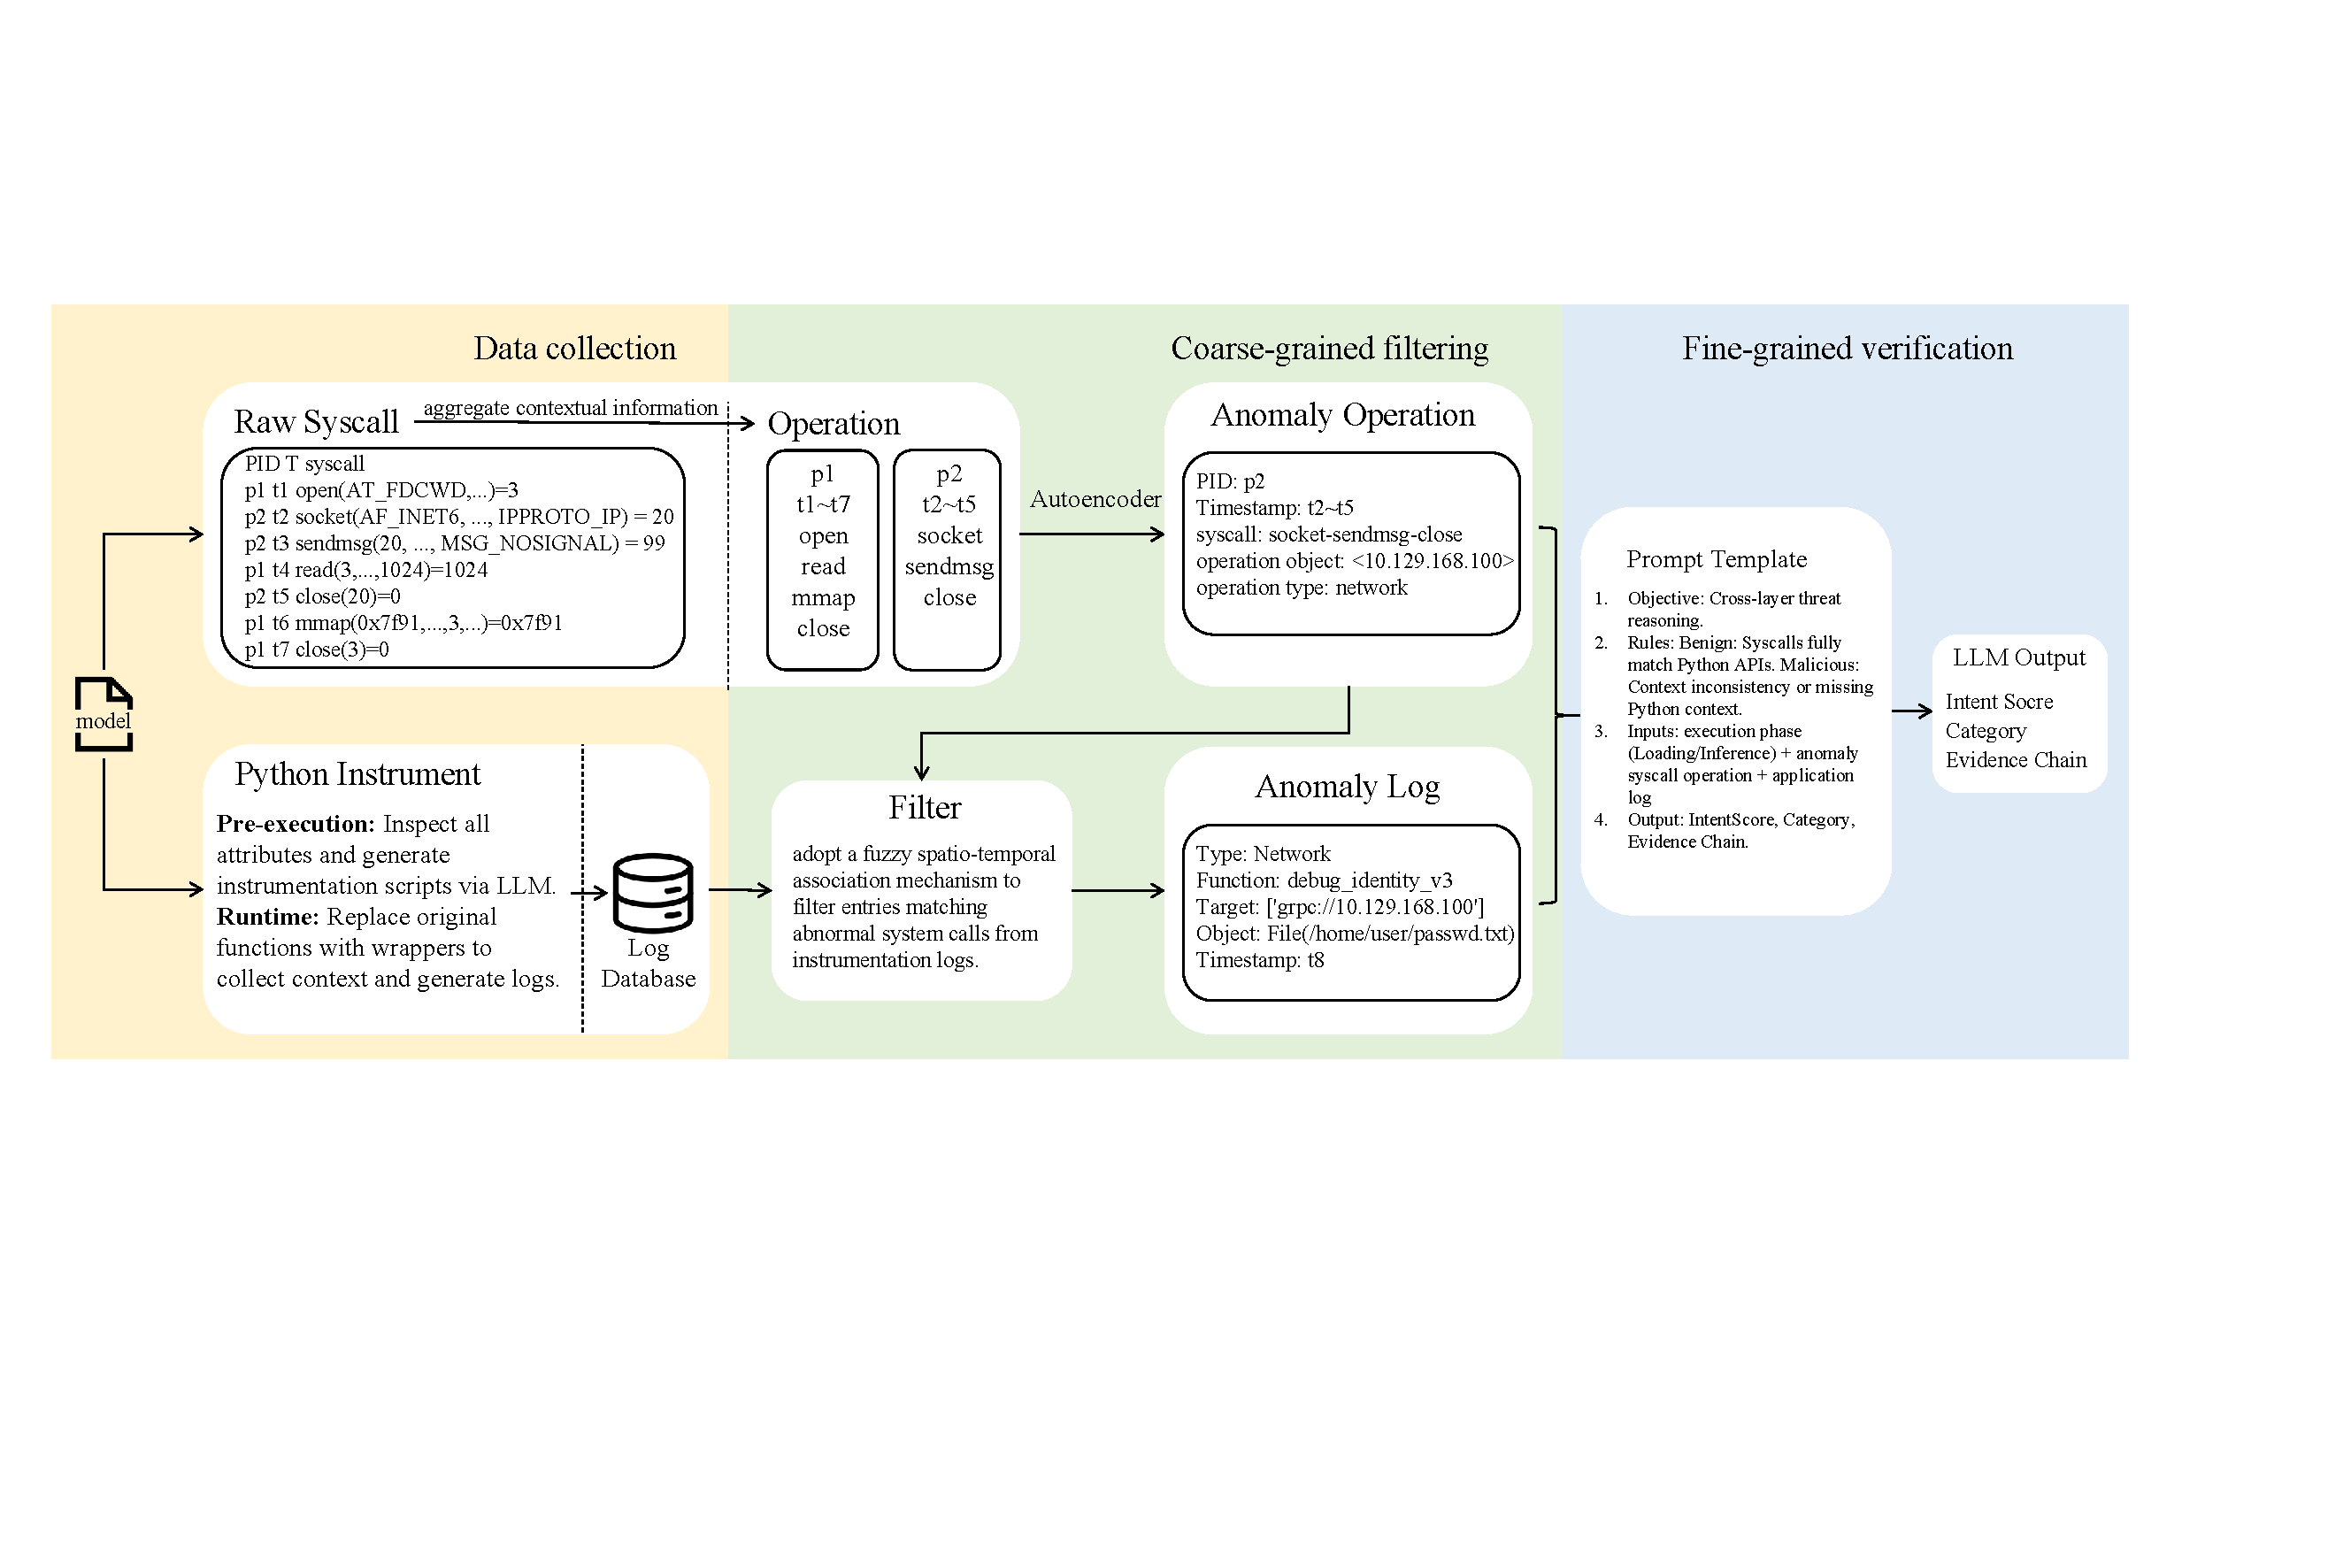
\includegraphics[width=\linewidth]{figs/overview3.pdf}
    \caption{Overview of the hybrid defense system.}
    \label{fig:overview}
\end{figure*}

\subsection{Data Collection}

The data collection stage simultaneously captures two synchronized streams of evidence during controlled model execution: a kernel-visible system-call stream and an application-layer semantic log stream. Together, these streams provide the complementary low-level and high-level signals needed for downstream analysis.

\subsubsection{System-call collection.}
We base our detection on system-call traces because they operate below the user-space level and cannot be bypassed by any Python-level obfuscation~\cite{2875487}: no matter how a model artifact hides its malicious intent through code mangling or dynamic loading, its actual interactions with the operating system must traverse the kernel and therefore leave a non-bypassable forensic record.

\begin{table}[t!]
	\centering
	\caption{Security-relevant system-call categories used by our filter.}
	\begin{tabular}{l p{0.28\columnwidth} p{0.45\columnwidth}}
		\hline
		Filter param & Category & Purpose \\
		\hline
		file   & File operations (\texttt{read}/\texttt{write}) & Detect sensitive data leakage or configuration file tampering \\
		network & Network operations (\texttt{socket}) & Detect data exfiltration or remote command execution \\
		cred   & Credential operations (\texttt{setuid}) & Detect privilege-escalation behavior \\
		desc   & Descriptor operations (\texttt{dup}) & Assist file-related anomaly detection \\
		signal & Signal handling (\texttt{kill}) & Capture malicious process termination attempts \\
		clock  & Time-related operations & Assist temporal anomaly analysis (e.g., abnormal delays) \\
		\hline
	\end{tabular}
	\label{tab:syscalltypes}
\end{table}

We employ a selective tracing strategy that focuses exclusively on security-relevant system-call families, discarding high-frequency but semantically uninformative calls to keep the trace volume manageable. During controlled model execution, we use \texttt{strace} to continuously trace system calls of the target process. To reduce noise and overhead, we immediately discard calls such as scheduler hints and memory-mapping operations that carry no security signal\cite{shakya2022analysisdetectionclassificationandroid}. The selection concentrates on system-call categories that can indicate malicious intent. Table~\ref{tab:syscalltypes} summarizes the security-relevant syscall families we monitor and their roles in our detection pipeline. For example, file operations can reveal attempts to access sensitive data or modify configurations, while network operations may signal data exfiltration or remote command execution.

\subsubsection{Instrumentation log collection.}
To bridge the semantic gap between model-level intent and kernel-level behavior, we collect high-dimensional Python semantic context via non-invasive instrumentation. The key challenge is that heterogeneous ML frameworks expose frequently changing APIs, making manual per-framework instrumentation labor-intensive and coverage-incomplete. We address this through an LLM-assisted approach with two distinct phases.

\noindent \textbf{Pre-execution: API Discovery and Script Generation.}
Before model execution, we leverage an LLM to synthesize dynamic instrumentation scripts. A rigorously structured prompt constrains the LLM to generate code that inspects the target module's namespace at startup, systematically identifies all public callable attributes, and constructs wrapper closures around each. The prompt specifies the security objective, mandates capturing execution context which contains timestamps, operation types, argument values and return types, and requires all intercepted events to be serialized into standardized JSON. This automated discovery eliminates statically hardcoded API lists and adapts to framework version changes by simply regenerating wrappers for the new API surface, without modifying the core detection pipeline.

Algorithm~\ref{alg:instrumentation} formalizes this discovery and wrapping logic. The \texttt{ApplyDynamicPatches} procedure isolates public callables while skipping private attributes and non-callable objects, then generates wrapper closures for each target API.

\begin{algorithm}[t!]
\caption{Automated Dynamic Instrumentation Logic}
\label{alg:instrumentation}
\KwIn{Target library module $\mathcal{M}$ (e.g., \texttt{torch}, \texttt{tensorflow})}
\KwOut{Instrumented module capable of context logging}

\SetKwProg{Fn}{Procedure}{:}{}
\SetKwFunction{FApply}{ApplyDynamicPatches}
\SetKwFunction{FConstruct}{Wrapper}

\Fn{\FApply{$\mathcal{M}$}}{
    \ForEach{attribute name $attr\_name$ \textnormal{\textbf{in}} \textnormal{dir}($\mathcal{M}$)}{
        \If{$attr\_name$ starts with ``\_''}{
            \textbf{continue} 
        }
        
        $target\_func \gets$ \textnormal{getattr}($\mathcal{M}, attr\_name$)\;
        \If{\textnormal{\textbf{not}} is\_callable($target\_func$)}{
            \textbf{continue} 
        }
        
        $wrapper \gets$ \FConstruct{$target\_func, attr\_name$}\;
        
        \textbf{try}\;
        \Indp \textnormal{setattr}($\mathcal{M}, attr\_name, wrapper$)\; 
        \Indm \textbf{catch} \textit{ReadOnlyAttributeError} \;
        \Indp \textbf{continue} \;
        \Indm
    }
}
\Fn{\FConstruct{$func, name$}}{
    \KwRet a closure that captures the full \texttt{traceback}, logs to JSON, executes $func$, and delegates return value\;
}
\end{algorithm}

\noindent \textbf{Runtime: Wrapper Injection and Context Logging.}
At process startup, the generated script employs monkey patching (\texttt{setattr}) to replace original functions with wrapper closures. Thereafter, any invocation of a wrapped API triggers the injected closure, which captures the execution context and serializes it as a structured semantic event:
\begin{equation}
\ell_i = \langle \textit{FuncName},\; \textit{ArgsSummary} \rangle.
\end{equation}
Here $\textit{FuncName}$ denotes the invoked framework or standard-library API, while $\textit{ArgsSummary}$ aggregates only lightweight information—tensor shapes and dtypes, configuration flags, truncated or hashed file paths, and bounded-length string summaries—controlling logging overhead while preserving rich contextual signals.

To ensure runtime safety, wrappers follow a conservative policy: they only wrap callable functions avoiding class definitions, built-in types, and C/C++ bindings, perform best-effort argument summarization without altering return values or side effects, and employ defensive serialization. The patching process is additionally wrapped in \texttt{try-except} blocks to survive read-only properties, immutable C-extension bindings, and dynamically generated descriptors that would otherwise crash the process. Any patch failure degrades gracefully without disrupting the target process.

\subsection{Coarse-grained Filtering}

After collecting raw evidence streams, the coarse-grained filtering stage transforms system-call traces into compact operation vectors, screens for anomalies, and retrieves the corresponding semantic context. This stage eliminates clearly benign activity before the expensive LLM reasoning stage.

\subsubsection{System-call Clustering and Embedding}

The collected system-call traces are extremely fine-grained and voluminous. A single model loading process may produce thousands of system calls, and meaningful malicious behavior invariably manifests as a \emph{sequence} of related calls rather than as isolated events. To address this, we aggregate correlated system calls into compact, high-level operation vectors that reduce trace noise, compress data volume, and provide standardized analysis units with complete semantics for downstream anomaly detection.

To accurately model the execution semantics of a program, it is crucial to recognize that system calls inherently possess varying degrees of contextual dependency. Applying a uniform extraction strategy to all system calls would be ineffective: some operations are semantically self-contained and immediately indicative of high-risk behavior, whereas others are granular, stateful operations that remain ambiguous unless analyzed as a continuous sequence. Motivated by this fundamental difference, we propose a hybrid embedding scheme that categorizes the traced system calls into two distinct streams for targeted handling: (1) \emph{Directly malicious calls} and (2) \emph{Stateful calls}. By processing these two streams individually, we ultimately synthesize them into a unified feature space for downstream analysis.

\noindent \textbf{Direct call embedding.}
The first category includes standalone, high-risk operations (e.g., \texttt{execve}, \texttt{chmod}) that do not require lifecycle context. We directly encode each of these calls into a fixed-dimension operation vector $\mathbf{v}_{\textit{dir}} \in \mathbb{R}^{d}$. Specifically, we utilize a pre-trained BERT-based model to extract the rich semantic meaning from the call's underlying logic and literal arguments. This high-dimensional representation is subsequently projected down to the target dimension $d$, ensuring that semantically critical, self-contained threats are instantly captured without the need for sequence aggregation.

\noindent \textbf{Stateful aggregation.}
Let $S = \{(s_k, \tau_k)\}_{k=1}^{N}$ denote the traced system-call stream, where $s_k$ is the $k$-th syscall and $\tau_k$ its timestamp. For stateful operations, we maintain per-resource state keyed by $r = \langle \textit{PID}, \textit{FD} \rangle$, where $\textit{FD}$ denotes a file or socket descriptor. For each key $r$, we collect the indices of calls that operate on this resource within one lifecycle segment,
\begin{equation}
I_r = \{\, k \mid (s_k, \tau_k) \in S,\ s_k \text{ uses resource } r,\ \tau_{\textit{start}}^r \le \tau_k \le \tau_{\textit{end}}^r \,\},
\end{equation}
where $\tau_{\textit{start}}^r$ and $\tau_{\textit{end}}^r$ are the timestamps of the resource-acquisition and resource-release calls (e.g., \texttt{open} / \texttt{close} or \texttt{socket} / \texttt{shutdown}). The lifecycle segment for resource $r$ is then the ordered subsequence $S_r = \{(s_k, \tau_k)\}_{k \in I_r}$.

We aggregate this segment into a fixed-length operation vector by applying a feature-extraction function $\phi$ over all calls in the segment:
\begin{equation}
\mathbf{v}_{\textit{sys}}(r) = \phi(S_r) \in \mathbb{R}^{d},
\end{equation}
where $\phi$ operates by extracting the common resource identifier $r = \langle \textit{PID}, \textit{FD} \rangle$ shared across the segment $S_r$, and concatenating it with the sequence of distinct, call-specific parameters (e.g., flags, buffer sizes, or return values) derived from each individual system call $s_k \in S_r$. This concatenated feature sequence is subsequently passed through an embedding layer to project it into the continuous $\mathbb{R}^{d}$ space. Intuitively, each $\mathbf{v}_{\textit{sys}}(r)$ captures a dense, contextualized representation of the exact data flow and state transitions associated with a specific file or connection during its lifetime, effectively smoothing out scheduling artifacts and interleaving from other threads.

The final feature matrix combines $\mathbf{v}_{\textit{dir}}$ and $\mathbf{v}_{\textit{sys}}$, enabling the system to capture both direct and aggregated syscall behaviors. This hybrid representation ensures that directly malicious actions are immediately flagged, while stateful operations are analyzed in context to detect more subtle threats.

\subsubsection{Autoencoder-based Anomaly Detection}

We adopt unsupervised anomaly detection because benign model loading and inference produce a stable, learnable distribution of system-call operations, whereas malicious behaviors are inherently rare and diverse, making supervised classification impractical without labeled attack samples that cover the full threat space. Among unsupervised methods, we choose an Autoencoder for its conceptual simplicity and proven effectiveness in reconstruction-based anomaly detection: it learns to faithfully reconstruct benign operation vectors during training and naturally flags any vector it cannot faithfully reconstruct as anomalous.

We train an Autoencoder on operation vectors collected from clean model loading and inference runs. Given an operation vector $\mathbf{v}$, the Autoencoder computes a reconstruction error
\begin{equation}
E = \left\lVert \mathbf{v} - \textit{Dec}(\textit{Enc}(\mathbf{v})) \right\rVert_2^2,
\end{equation}
where \textit{Enc} and \textit{Dec} denote the encoder and decoder networks, respectively. Operations with reconstruction error $E$ below a threshold $\theta$ are treated as consistent with normal model behavior and are discarded. If $E > \theta$, we mark the corresponding operation as abnormal, retain its full underlying system-call segment $S'$ and metadata $\langle \textit{PID}, \textit{TID}, t_{\textit{start}}, t_{\textit{end}} \rangle$, and promote it to the subsequent spatio-temporal matching stage.

By performing this unsupervised prefiltering at the operation level, the system keeps the expensive cross-layer association and LLM reasoning off the critical path for the vast majority of benign activity, while still surfacing rare, suspicious low-level behaviors that deviate from the learned distribution of normal AI model execution.

\subsubsection{Spatio-temporal Semantic Matching}

After the autoencoder identifies abnormal operations, we must determine whether each anomaly can be explained by benign Python-level behavior. This requires retrieving the semantic context from the instrumentation log stream that corresponds to each abnormal system-call operation.

System calls and Python semantics are inherently asynchronous due to operating system scheduling and concurrent I/O. As a result, naive one-to-one timestamp matching between system-call logs and semantic logs is unreliable in high-concurrency workloads. We therefore adopt a fuzzy spatio-temporal association strategy.

For each abnormal operation, the autoencoder screening stage provides the underlying system-call segment $S'$ and its metadata $\langle \textit{PID}, t_{\textit{start}}, t_{\textit{end}} \rangle$. Given this metadata and the semantic log stream $L = \{(\ell_i, t_i)\}$, we perform filtering following the spatial-temporal matching rules below.

\noindent \textbf{Temporal windowing.}
We apply a slack temporal window around the abnormal operation. For each candidate abnormal operation, we define its active time span $[t_{\textit{start}}, t_{\textit{end}}]$ based on the first and last system call in $S'$, and search semantic events whose timestamps $t_i$ fall into an expanded window $[t_{\textit{start}} - \Delta t, t_{\textit{end}} + \Delta t]$. The slack parameter $\Delta t$ tolerates minor scheduling jitter while still localizing semantic context to the period when the resource was actually in use.

\noindent \textbf{Spatial hints.}
Temporal proximity alone is insufficient under heavy concurrency. We therefore further filter candidates using resource-related hints derived from both layers, such as whether the operation is file- or network-related, file paths or prefixes, remote destinations, and other descriptor metadata when available. Combining temporal and spatial constraints yields a fuzzy but robust alignment that significantly reduces spurious associations when many model components execute in parallel.

\subsection{Fine-grained Verification}

Operations that survive coarse-grained filtering are escalated to the fine-grained verification stage, which jointly reasons about the low-level system-call evidence and high-level semantic context to produce a final intent judgment.

Determining whether abnormal low-level operations reflect benign model behavior or malicious intent is inherently challenging: the same system-call pattern can arise from legitimate model loading or from an attacker's attempt to exfiltrate data, and without semantic context the two are indistinguishable at the kernel level. To resolve this ambiguity, we feed each abnormal operation together with its aligned semantic contexts into an LLM, which judges whether the behavior is consistent with benign model execution.

\noindent \textbf{Prompt construction.}
We translate the aligned evidence into a structured natural-language prompt that includes: (i) a concise summary of the abnormal operation including operation type, key statistics, and risk-relevant parameters, (ii) the aligned semantic call contexts including library/API, call stack summary, and argument summaries, and (iii) the execution phase categorized into the model loading stage and inference stage.

Our maliciousness judgment follows a principled cross-layer reasoning rule: a behavior is classified as benign only when its low-level system-call activity can be plausibly explained by the aligned Python-level semantic context. Concretely, if the LLM identifies that the observed file reads, network connections, or process creations are consistent with the framework APIs and execution phase reported in the semantic log, the operation is deemed benign and discarded. Conversely, when inconsistencies exist between the Python-layer semantic logs and the corresponding system-call activities, such as a network connection to an external host with no matching high-level API invocation, or when no matching Python semantic context can be retrieved at all, the behavior is marked as malicious and escalated.

\noindent \textbf{Decision and explanation.}
The LLM outputs $\textit{IntentScore}$, a $\textit{ThreatCategory}$ label, and a rationale. Importantly, we persist the subset of semantic events and system-call summaries used in the reasoning as the \emph{evidence chain} $\textit{Context}$ for auditing.
If high-risk system-call patterns appear without any plausible semantic explanation, the system raises a high-severity alert and can block execution in the controlled environment.


\subsection{Model Vetting Pipeline}
%% [Deployment: \toolname{} operates in pre-deployment fuzzing pipeline, not production serving]

\toolname{} is designed to operate in a pre-deployment model vetting pipeline rather than in production inference serving. Before a model is released or integrated into any production system, it should undergo a comprehensive security vetting phase in a controlled sandbox environment with \toolname{} monitoring its behavior to detect embedded malicious logic.

To maximize detection coverage, we recommend exhaustive fuzzing-based testing of all real-world business workflows that the model will encounter post-deployment\cite{wu2026chainfuzzergreyboxfuzzingworkflowlevel, BAMOHABBATCHAFJIRI2024103903}. Concretely, the model should be exercised through every anticipated usage scenario: loading with all expected input shapes and data types, invoking inference across the full range of supported batch sizes, exercising all serialization, checkpointing, and fine-tuning paths, and simulating edge-case inputs that stress runtime boundaries. This fuzzing strategy ensures that dormant malicious payloads—which may be conditionally triggered only under specific runtime conditions, input patterns, or execution phases—are activated and exposed during testing, providing comprehensive coverage beyond simple model loading.

\section{Evaluation}\label{sec:evaluation}

We evaluate the effectiveness of \toolname{} in detecting malicious behavior embedded in model artifacts. We organize the evaluation around the following research questions:

\begin{itemize}[noitemsep, topsep=1pt, partopsep=1pt, listparindent=\parindent, leftmargin=*]
    \item \textbf{RQ1:} What is the performance of \toolname{} in detecting malicious models, and does it show significant advantages over the baselines?
    \item \textbf{RQ2:} What is the runtime overhead of \toolname{}, and is it practical to deploy in real-world model workflows?
    \item \textbf{RQ3:} How does each part of \toolname{} contribute to the detection performance?
\end{itemize}


\subsection{Experiment Setup}

\noindent \textbf{Datasets.}
We evaluate \toolname{} on two datasets spanning known deserialization exploits and advanced framework-native attacks:
\begin{itemize}
    \item \emph{MalHug Dataset.} 89 models identified as anomalous by MalHug from public repositories. Manual source code auditing and sandbox verification label 78 as malicious—mainly abusing Pickle deserialization to implant reverse shells—and 11 as benign proof-of-concept samples that verify exploitability without destructive operations. While these represent real-world threats, their methodologies rely on well-known deserialization flaws and are straightforward to detect with existing static scanners.
    \item \emph{Advanced TensorAbuse Synthetic Dataset.} To evaluate our system against highly stealthy, framework-native attacks, we constructed a second dataset using the TensorAbuse framework~\cite{zhu2025}. This corpus comprises two complementary subsets. The \textbf{malicious subset} contains 80 models: for each of 10 diverse foundation models, we embed 8 attack variants spanning four categories using TensorAbuse primitives. The complete catalog of primitive APIs and the attack composition procedure are detailed in Appendix~\ref{appendix:dataset}. The \textbf{Benign Subset} contains 40 models that invoke the same high-risk native TensorFlow APIs for legitimate purposes such as outputting debug tags, constructed to precisely quantify the false-positive rate. 
\end{itemize}

For all datasets, the model artifact is the unit under test. Labels are assigned by manual payload inspection.

\noindent \textbf{Baselines.}
We compare against four baseline detection methods: three widely adopted security scanners integrated into the Hugging Face platform—JFrog~\cite{jfrog2024huggingface}, Protect AI~\cite{modelscan}, and ClamAV~\cite{clamav}—and the specialized detection tool from TensorAbuse~\cite{zhu2025}.
For JFrog, Protect AI, and ClamAV, we uploaded our model artifacts to the Hugging Face platform, triggering its live security scanning pipelines to capture authentic detection efficacy in a real-world supply chain setting. For TensorAbuse, we use the authors' open-source implementation. 

All experiments run on a workstation with dual Intel Xeon Silver 4210R CPUs, 128 GB RAM, and two NVIDIA GeForce RTX 3090 GPUs.

\subsection{RQ1: Detection Performance}

%To answer RQ1, we compare \toolname{} with the baselines on the curated malicious corpus and synthetic variants. For each model, we execute a standardized loading and inference procedure in a sandbox and record whether the detector raises an alert. We measure \emph{detection rate} (true positive rate on malicious models), \emph{false-positive rate} (fraction of benign models flagged as malicious), and \emph{precision}.

%Empirically, static scanners achieve high precision on simple payloads that explicitly import dangerous APIs, but miss a substantial fraction of attacks that hide behind authorized interfaces or deferred execution. System-call-only baselines detect a larger fraction of attacks, especially those that perform overt file or network operations, but suffer from elevated false positives on benign models with unusual I/O patterns (e.g., heavy checkpointing or remote logging).

%\toolname{} consistently achieves higher detection rates than static scanners while maintaining a lower false-positive rate than the system-call-only baseline. By combining unsupervised low-level anomaly detection with cross-layer intent reasoning, \toolname{} successfully flags camouflage attacks that are deliberately structured to evade static signatures, yet avoids over-flagging benign utilities that legitimately exercise advanced framework features.
\label{sec:rq1}

%% [ORIGINAL INTRO -- commented for restructuring]
%To answer this research question, we evaluate the detection performance of \toolname{} and the baseline methods across both the in-the-wild malicious model dataset from MalHug and our advanced TensorAbuse synthetic corpus. This comprehensive evaluation demonstrates \toolname{}'s effectiveness in identifying a wide spectrum of malicious activities, ranging from known deserialization exploits to sophisticated framework-native attacks.

To answer this research question, we evaluate the detection performance of \toolname{} and the baseline methods across both datasets. 

\begin{table}[t!]
    \scriptsize
    \centering
    \caption{Detection performance of \toolname{} and baselines across both datasets.}
    \resizebox{0.49\textwidth}{!}{\begin{tblr}{
        cell{1}{1-7} = {c},
        cell{2-7}{2-7} = {c},
        vline{2,5},
        hline{1,2,8} = {1pt},
        stretch=0
    }
    \SetCell[r = 2, c = 1]{c} \textbf{Method} & \SetCell[r = 1, c = 3]{c} \textbf{MalHug} & & & \SetCell[r = 1, c = 3]{c} \textbf{Advanced TensorAbuse Synthetic} & & \\
    & \textbf{Precision} & \textbf{Recall} & \textbf{F1} & \textbf{Precision} & \textbf{Recall} & \textbf{F1} \\ \hline
    \SetCell[r = 1, c = 1]{c} \textbf{JFrog} & 0.8953 & 0.9872 & 0.9390 & 0.8889 & 0.3750 & 0.5275 \\
    \SetCell[r = 1, c = 1]{c} \textbf{Protect AI} & 0.8966 & \textbf{1.0000} & 0.9455 & 0.7273 & 0.5000 & 0.5928 \\
    \SetCell[r = 1, c = 1]{c} \textbf{ClamAV} & 0.8904 & 0.8333 & 0.8609 & -- & 0.0000 & -- \\
    \SetCell[r = 1, c = 1]{c} \textbf{TensorAbuse} & -- & -- & -- & 0.6667 & \textbf{1.0000} & 0.8000 \\ \hline
    \SetCell[r = 1, c = 1]{c} \textbf{\toolname{}} & \textbf{1.0000} & 0.9744 & \textbf{0.9870} & \textbf{1.0000} & \textbf{1.0000} & \textbf{1.0000} \\
    \end{tblr} }
    \label{tab:combined_result}
\end{table}

%% [ORIGINAL OVERVIEW -- commented for restructuring]
%Table~\ref{tab:combined_result} provides an overview of detection performance across both datasets. Two contrasting patterns emerge. On the MalHug dataset, traditional static scanners achieve moderate-to-high F1 scores by matching known deserialization signatures, with \toolname{} marginally outperforming them through precise intent verification. On the Synthetic Corpus, however, the performance gap widens dramatically: static tools degrade sharply, while TensorAbuse's perfect recall is offset by a 0.6667 precision from its inability to distinguish legitimate TensorFlow API usage. Only \toolname{} maintains high performance on both datasets, achieving an F1 of 0.9870 on MalHug and a perfect 1.0000 on the Synthetic Corpus. We next analyze each dataset in detail.

Table~\ref{tab:combined_result} summarizes the detection performance across both datasets. On the MalHug Dataset, traditional static scanners achieve moderate to high F1 scores by matching known deserialization signatures. \toolname{} achieves a marginal improvement via accurate intent verification. However, on the Advanced TensorAbuse Synthetic Dataset, the performance gap expands dramatically. Static tools suffer a sharp drop in detection performance. While TensorAbuse achieves a perfect recall, its precision is only 0.6667, as it fails to distinguish legitimate and malicious calls to TensorFlow APIs. Only \toolname{} maintains consistently high performance on both datasets, achieving an F1 of 0.9870 on the MalHug Dataset and a perfect 1.0000 on the Advanced TensorAbuse Synthetic Dataset. We next analyze each dataset in detail.

%% [ORIGINAL MALHUG ANALYSIS -- commented for restructuring]
%\textbf{Performance on In-the-wild Dataset.} We first evaluate the methods on the dataset comprising 89 models in total, consisting of 78 genuinely malicious models and 11 benign proof-of-concept models. It is important to note that the attacks in this dataset primarily rely on inserting malicious payloads through insecure serialization vulnerabilities. Because this specific attack methodology is well-known and extensively studied, traditional static detection tools such as JFrog, Protect AI, and ClamAV achieve relatively high recall rates by relying on established vulnerability signatures. However, these baseline methods exhibit a critical limitation: they fail to distinguish between actual weaponized attacks and the 11 benign models. Detailed manual analysis revealed that these 11 models merely exploit the inherent mechanics of insecure serialization formats to execute normal operations, demonstrating the exploitability of the vulnerability as a proof-of-concept without performing genuinely harmful actions like data exfiltration or unauthorized network access. By simply classifying any model containing a vulnerable signature as malicious, these traditional methods generate significant false positives.
%
%In contrast, \toolname{} successfully detects 76 out of the 78 genuinely malicious models, while accurately categorizing all 11 proof-of-concept models as non-malicious. Because \toolname{} relies on a two-stage screening process that evaluates the actual intent of the dynamic behavior rather than merely matching static signatures, it demonstrates robust resilience against false positives. Finally, in stark contrast to all other methods, the TensorAbuse detection tool fails to identify any of these models, as its static graph-based approach cannot capture deserialization exploits that occur before or outside the computational graph instantiation.

\noindent \textbf{Performance on the MalHug Dataset.} Traditional static detection tools such as JFrog, Protect AI, and ClamAV achieve relatively high recall rates by relying on established vulnerability signatures. However, these baselines exhibit a critical limitation: they fail to distinguish actual weaponized attacks from the 11 benign proof-of-concept models. By simply classifying any model containing a vulnerable signature as malicious, these methods generate substantial false positives.

In contrast, \toolname{} successfully detects 76 out of 78 genuinely malicious models while accurately categorizing all 11 proof-of-concept models as non-malicious. Because \toolname{} evaluates the actual intent of dynamic behavior rather than merely matching static signatures, it demonstrates robust resilience against false positives. Notably, the TensorAbuse detector fails to identify any of these models, as its static graph-based approach cannot detect deserialization exploits triggered before computational graph initialization or outside the scope of the computational graph.

\begin{table}[t!]
    \scriptsize
    \centering
    \caption{Detected malicious models on the TensorAbuse Synthetic Dataset by attack type (20 per type).}
    \resizebox{0.49\textwidth}{!}{\begin{tblr}{
        cell{1-2}{1-6} = {c},
        cell{3-7}{2-6} = {c},
        vline{2},
        hline{1,8} = {1pt},
        stretch=0
    }

    \SetCell[r = 2, c = 1]{c} \textbf{Method} & \SetCell[r = 1, c = 4]{c} \textbf{Attack Type (Total models)} & & & & \SetCell[r = 2, c = 1]{c} \textbf{Total Detected} \\ \cline{2-5}
    & \textbf{File Exfil.} & \textbf{IP Exposure} & \textbf{Code Insertion} & \textbf{Remote Shell} & \\ \hline
    \textbf{JFrog}       & 20 / 20 & 0 / 20  & 0 / 20  & 10 / 20 & 30 / 80 \\
    \textbf{Protect AI}  & 20 / 20 & 0 / 20  & 0 / 20  & 20 / 20 & 40 / 80 \\
    \textbf{ClamAV}      & 0 / 20  & 0 / 20  & 0 / 20  & 0 / 20  & 0 / 80 \\
    \textbf{TensorAbuse} & \textbf{20} / 20 & \textbf{20} / 20 & \textbf{20} / 20 & \textbf{20} / 20 & \textbf{80} / 80 \\ \hline
    \textbf{\toolname{}}         & \textbf{20} / 20 & \textbf{20} / 20 & \textbf{20} / 20 & \textbf{20} / 20 & \textbf{80} / 80 \\
    \end{tblr} }
    \label{tab:synthetic_result}
\end{table}

%% [ORIGINAL SYNTHETIC ANALYSIS -- commented for restructuring]
%\textbf{Performance on Advanced Synthetic Corpus.} We further evaluate the methods on our rigorously constructed dataset of 80 advanced malicious models, where attacks are deeply embedded within the models' computational graphs. Table~\ref{tab:synthetic_result} provides a detailed breakdown of the detection results across the four distinct attack categories (File Leakage, IP Exposure, Malicious Code Insertion, and Remote Shell Acquisition). Both \toolname{} and the TensorAbuse detection tool successfully detect 100\% of the malicious models in this corpus. The TensorAbuse tool achieves perfect detection here because these specific attacks were generated using its own primitive methodologies, making them highly visible to its static API-checking mechanism. However, as demonstrated in Table~\ref{tab:combined_result}, its static approach fails entirely against attacks outside its predefined scope. 
%
%Conversely, \toolname{} achieves this 100\% detection rate without relying on static signatures or predefined API lists. By statistically profiling the benign baseline behaviors of models like BERT and VGG16, and dynamically intercepting the anomalous system calls generated by the malicious payloads such as unexpected network connections or file reads, \toolname{} accurately identifies the malicious intent regardless of the specific attack vector employed. The performance of the remaining baseline tools—JFrog, Protect AI, and ClamAV—varies significantly across the different attack categories, highlighting the limitations of traditional scanning tools when faced with sophisticated, framework-native manipulations.

\noindent \textbf{Performance on the Advanced TensorAbuse Synthetic Dataset.} Table~\ref{tab:synthetic_result} provides a detailed breakdown of the detection results. Both \toolname{} and the TensorAbuse detection tool successfully detect 100\% of the malicious models. The TensorAbuse tool achieves perfect detection here because these attacks were generated using its own primitive methodologies, making them highly visible to its static API-checking mechanism. However, as shown in Table~\ref{tab:combined_result}, its static approach fails entirely against attacks outside its predefined scope.

Conversely, \toolname{} achieves this 100\% detection rate without relying on static signatures or predefined API lists. By statistically profiling benign baseline behaviors of models and dynamically intercepting the anomalous system calls generated by malicious payloads, \toolname{} accurately identifies malicious intent regardless of the specific attack vector. The performance of JFrog, Protect AI, and ClamAV varies significantly across attack categories, highlighting the limitations of traditional scanning tools against sophisticated, framework-native manipulations.

To further verify \toolname{}'s capability against false positives, we also evaluate all methods on benign models.

% \begin{table}[h!]
%     \scriptsize
%     \centering
%     \caption{False Positive evaluation of \toolname{} and baselines on 40 benign models utilizing sensitive TensorFlow APIs. (Lower is better.)}
%     \resizebox{0.49\textwidth}{!}{\begin{tblr}{
%         cell{1}{1-2} = {c},
%         cell{2-6}{2} = {c},
%         vline{2},
%         hline{1,7} = {1pt},
%         stretch=0
%     }
%     \SetCell[r = 1, c = 1]{c} \textbf{Method} & \SetCell[r = 1, c = 1]{c} \textbf{False Positives / Total Benign (FPR)} \\ \hline
%     \SetCell[r = 1, c = 1]{c} \textbf{JFrog} & 10 / 40 (25.00\%) \\
%     \SetCell[r = 1, c = 1]{c} \textbf{Protect AI} & 30 / 40 (75.00\%) \\
%     \SetCell[r = 1, c = 1]{c} \textbf{ClamAV} & \textbf{0} / 40 (\textbf{0.00\%}) \\
%     \SetCell[r = 1, c = 1]{c} \textbf{TensorAbuse} & 40 / 40 (100.00\%) \\ \hline
%     \SetCell[r = 1, c = 1]{c} \textbf{\toolname{}} & \textbf{0} / 40 (\textbf{0.00\%}) \\
%     \end{tblr} }
%     \label{tab:benign_result}
% \end{table}

The precision results on the Advanced TensorAbuse Synthetic Dataset in Table~\ref{tab:combined_result} clearly reveal the drawbacks of static detection mechanisms. TensorAbuse misclassifies all 40 benign models as malicious, resulting in a 100\% false positive rate. It relies solely on static scanning against a predefined blacklist of high-risk APIs and lacks the ability to understand API semantics and invocation context. Similarly, JFrog and Protect AI also produce numerous misclassifications, indicating that signature-based detection methods fail when legitimate operations overlap with known attack patterns.

In contrast, \toolname{} successfully identifies all 40 models as benign. By dynamically observing runtime execution, \toolname{}'s first stage recognizes that the system calls generated by these APIs align with the established statistical baseline of normal framework operations. When a suspicious operation triggers cross-layer analysis, the LLM-based reasoning engine interprets high-level Python semantics to validate benign intent. This demonstrates that \toolname{} bridges the semantic gap, providing accurate defense without impeding legitimate workflows.

%% [ORIGINAL CONCLUSION AND OLD RQ2 BENIGN CONTENT -- archived for reference]
%Overall, the results across both datasets demonstrate that \toolname{} provides a robust, highly generalizable defense mechanism capable of accurately detecting malicious AI model artifacts, regardless of whether they employ common deserialization flaws or advanced, stealthy computational graph manipulations.
%
%%\label{sec:rq2}
%% \subsection{RQ2: Benign Model Distinction.}
%
%While achieving a high detection rate is crucial, a practical defense system must not disrupt normal AI operations by aggressively flagging legitimate models. To answer this research question, we evaluate the false positive rates of \toolname{} and the baseline methods against a rigorously constructed dataset of benign models.
%
%\begin{table}[h!]
%    \scriptsize
%    \centering
%    \caption{False Positive evaluation of \toolname{} and baselines on 40 benign models utilizing sensitive TensorFlow APIs. (Lower is better.)}
%    \resizebox{0.49\textwidth}{!}{\begin{tblr}{
%        cell{1}{1-2} = {c},
%        cell{2-6}{2} = {c},
%        vline{2},
%        hline{1,7} = {1pt},
%        stretch=0
%    }
%    \SetCell[r = 1, c = 1]{c} \textbf{Method} & \SetCell[r = 1, c = 1]{c} \textbf{False Positives / Total Benign (FPR)} \\ \hline
%    \SetCell[r = 1, c = 1]{c} \textbf{JFrog} & 10 / 40 (25.00\%) \\
%    \SetCell[r = 1, c = 1]{c} \textbf{Protect AI} & 30 / 40 (75.00\%) \\
%    \SetCell[r = 1, c = 1]{c} \textbf{ClamAV} & \textbf{0} / 40 (\textbf{0.00\%}) \\
%    \SetCell[r = 1, c = 1]{c} \textbf{TensorAbuse} & 40 / 40 (100.00\%) \\ \hline
%    \SetCell[r = 1, c = 1]{c} \textbf{\toolname{}} & \textbf{0} / 40 (\textbf{0.00\%}) \\
%    \end{tblr} }
%    \label{tab:benign_result}
%\end{table}
%
%\textbf{Dataset Construction and Justification.} To rigorously stress-test the systems, we constructed a dataset of 40 entirely benign models. Crucially, these models were explicitly designed to incorporate the specific TensorFlow APIs such as \texttt{tf.raw\_ops.ReadFile} or \texttt{tf.io.matching\_files} that were identified as potential attack vectors in the TensorAbuse methodology. However, rather than weaponizing these APIs, we utilized them strictly for their intended, legitimate purposes—such as reading local dataset configurations, logging debug identities, or performing normal tensor persistence. It is important to emphasize that these are officially supported APIs provided by the TensorFlow standard library. Consequently, developers frequently rely on them in real-world scenarios for complex model training and inference pipelines. Thus, our dataset provides a highly realistic benchmark for evaluating whether a detection tool can understand the context of an API call rather than merely reacting to its presence.
%
%\textbf{Performance Analysis.} The false positive results are presented in Table~\ref{tab:benign_result}. The findings starkly illustrate the limitations of static, knowledge-dependent detection mechanisms. The TensorAbuse detection tool misclassifies all 40 benign models as malicious, resulting in a 100\% False Positive Rate (FPR). Because its detection logic inherently relies on statically scanning the computational graph for a predefined blacklist of "dangerous" APIs, it completely lacks the semantic awareness to differentiate between a legitimate data load and a malicious file exfiltration. Similarly, the traditional scanning tools—JFrog, Protect AI, and ClamAV—misclassify a portion of these models (-/-), further demonstrating that signature-based methods struggle when benign operations overlap with known attack heuristics.
%
%In contrast, \toolname{} successfully identifies all 40 models as benign, achieving a perfect 0.00\% FPR. By dynamically observing the runtime execution, \toolname{}'s first stage recognizes that the system calls generated by these APIs align with the established statistical baseline of normal framework operations. Even if a specific operation triggers a cross-layer analysis, the LLM-based reasoning engine in the second stage successfully interprets the high-level Python semantics to validate the benign intent. This demonstrates that \toolname{} successfully bridges the semantic gap, providing an exceptionally accurate defense mechanism that secures the supply chain without impeding legitimate developer workflows.

Overall, experimental results on both datasets prove that \toolname{} is a robust defense solution with strong generalization capability. It accurately detects malicious AI models exploiting common deserialization vulnerabilities or sophisticated computational graph tampering. Furthermore, equipped with cross-layer semantic reasoning, \toolname{} effectively differentiates legitimate usage of sensitive framework APIs from malicious attacks, achieving high precision on both datasets without interfering with developers' regular workflows.

\label{sec:rq2}
\subsection{RQ2: Efficiency and Deployability}

To evaluate the practical deployability of \toolname{}, we investigate its impact on host system performance and responsiveness to threats. We do not compare \toolname{} with the baseline methods here, as the baselines are strictly static analysis tools designed to scan model artifacts pre-deployment, whereas \toolname{} is a dynamic, runtime defense mechanism. Comparing the one-time scanning duration of static tools against the continuous runtime overhead of a dynamic monitor is fundamentally inequitable. Therefore, our evaluation focuses on the absolute performance impact of \toolname{} on standard model execution.

We assess efficiency using two primary metrics:
\begin{itemize}
    \item \emph{Performance Overhead:} The degradation in model loading time and inference throughput (Samples/Second) caused by deploying \toolname{}.
    \item \emph{Detection Latency:} The time elapsed from the exact moment a malicious operation is initiated by the model to the generation of the final alert.
\end{itemize}
\begin{table}[t!]
    \scriptsize
    \centering
    \caption{Runtime overhead and detection latency of \toolname{}.}
    \resizebox{0.49\textwidth}{!}{\begin{tblr}{
        cell{1-2}{1-6} = {c}, 
        cell{3-7}{2-6} = {c}, 
        vline{2},
        hline{1,8} = {1pt},
        stretch=0
    }
    \SetCell[r = 2, c = 1]{c} \textbf{Model} & \SetCell[r = 1, c = 3]{c} \textbf{Execution Time (s)} & & &  \textbf{Detection} \\ \cline{2-4}
    & \textbf{Vanilla} & \textbf{w/ MAD} & \textbf{Overhead} & \textbf{Latency (s)} \\ \hline
    \textbf{BERT}         & 11.4857 & 12.1767 & 6.02 \% & 13.5014 \\
    \textbf{YamNet}         & 16.3302 & 17.1434 & 4.98 \% & 10.3641 \\
    \textbf{EfficientNet} & 24.4290 & 25.8889 & 5.97 \% & 6.5911 \\
    \textbf{VGG16}        & 25.0444 &  26.4766 & 5.46 \% & 8.7171 \\ \hline
    \textbf{Average}      & 19.3223 & 20.4214 & 5.69 \% & 9.7934 \\
    \end{tblr} }
    \label{tab:overhead_result}
\end{table}

\begin{figure}[t!]
    \centering
    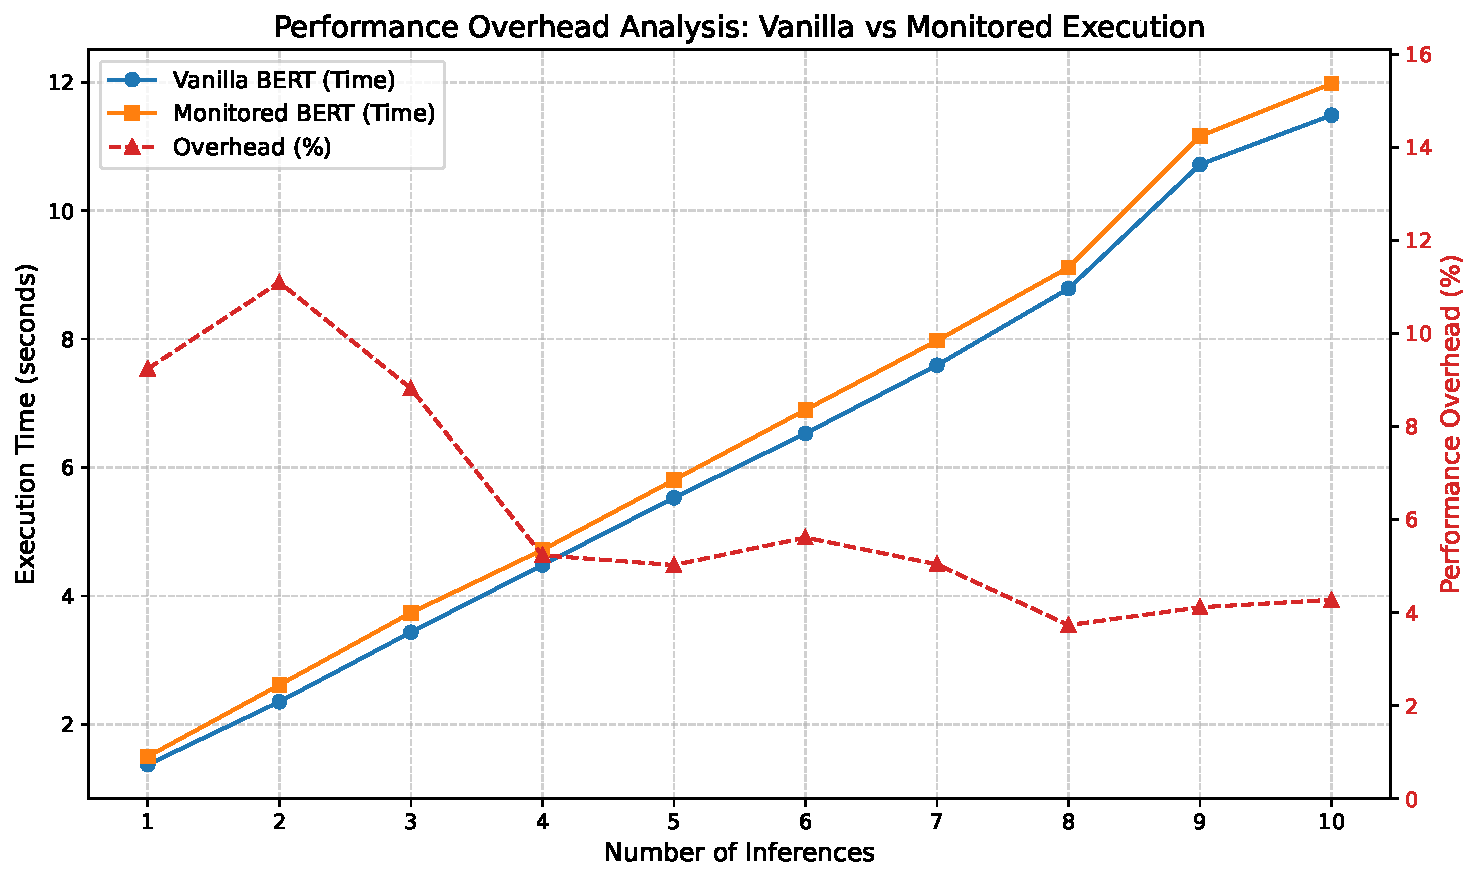
\includegraphics[width=0.45\textwidth]{figs/inference_overhead.pdf}
    \caption{Execution time of Vanilla vs.\ Monitored BERT and relative overhead across inferences.}
    \label{fig:inference_overhead}
\end{figure}


\textbf{Performance Overhead Analysis.} The performance impact of \toolname{} on normal model execution is presented in Table~\ref{tab:overhead_result}. \toolname{} introduces marginal overhead: the total execution time increases by an average of only 5.69\%, with the overhead consistently remaining within a narrow 4.9\% to 6.0\% margin across fundamentally different model architectures.

This performance penalty is attributed to our architectural design. First, the application-layer dynamic instrumentation employs a lightweight boundary-hooking mechanism that only captures high-level metadata instead of deeply traversing and serializing complex, multi-gigabyte Tensor objects. More importantly, the Autoencoder screening module and the \ac{llm} reasoning module run entirely asynchronously on the CPU. Because they do not compete for GPU memory or compute cycles, the intensive matrix multiplications and data parallelism required for AI inference remain completely unhindered.

To further demonstrate that our detection system minimally impacts inference efficiency, we analyzed the relationship between the number of inference iterations and relative latency overhead. Figure~\ref{fig:inference_overhead} illustrates the execution time of the BERT model over 1 to 10 inference steps, comparing vanilla execution with \toolname{}-monitored execution. The relative overhead percentage is highest during the initial executions but quickly drops and stabilizes at a lower baseline as the number of inferences increases.

This phenomenon aligns with the operating characteristics of deep learning frameworks. The model loading and initialization phases generate a large number of intensive system calls, such as memory mapping operations and heavy file I/O for loading model weights, which incur temporary CPU-bound monitoring overhead. However, once the model enters the continuous inference phase, intensive computations are primarily offloaded to hardware accelerators. These computations generate very few new system calls and do not occupy main CPU resources. Therefore, the overhead introduced by dynamic instrumentation and system call monitoring gradually diminishes.

\textbf{Detection Latency Analysis.} As shown in Table~\ref{tab:overhead_result}, \toolname{} achieves an average detection latency of 9.79 seconds. This latency encompasses the full analytical pipeline: capturing low-level system calls, completing the Autoencoder forward pass, extracting the corresponding Python contextual logs, and generating the final \ac{llm} intent classification. The \ac{llm} intent classification is only invoked on a small fraction of operations marked as abnormal by the Autoencoder, so its cost does not scale with total runtime but solely with the number of suspicious events.

While dynamic reasoning inherently introduces some delay compared to simple signature matching, this two-stage design keeps the overall overhead well within the acceptable budget for offline model vetting pipelines and pre-deployment security checks. 

\label{sec:rq3}

\subsection{RQ3: Component Ablation and Sensitivity}
In this section, we evaluate the contribution of each core component of \toolname{} through ablation studies. To demonstrate the necessity of our two-stage cross-layer architecture, we evaluate two variants:

\begin{itemize}
    \item \emph{\toolname{}--S}: which removes the unsupervised Autoencoder screening stage, directly feeding all raw system call windows and application-level instrumentation logs to the \ac{llm} for anomaly detection;
    \item \emph{\toolname{}--L}: which removes the application-level dynamic instrumentation, relying solely on the anomalous system call operations to make its final judgment;
\end{itemize}

\begin{table}[t!]
    \scriptsize
    \centering
    \caption{Ablation study of \toolname{}.}
    \resizebox{0.49\textwidth}{!}{\begin{tblr}{
        cell{1}{1-6} = {c},
        cell{2-4}{2-6} = {c},
        vline{2},
        hline{1,5} = {1pt},
        stretch=0
    }
    \SetCell[r = 1, c = 1]{c} \textbf{Method} & \SetCell[r = 1, c = 1]{c} \textbf{Precision} & \SetCell[r = 1, c = 1]{c} \textbf{Recall} & \SetCell[r = 1, c = 1]{c} \textbf{F1} & \SetCell[r = 1, c = 1]{c} \textbf{Latency (s)} & \SetCell[r = 1, c = 1]{c} \textbf{Token Cost} \\ \hline
    \SetCell[r = 1, c = 1]{c} \textbf{\toolname{}-S} & 90.91\% & 44.30\% & 59.57\% & 30.3126 & 867075 \\
    \SetCell[r = 1, c = 1]{c} \textbf{\toolname{}-L} & 85.25\%   & \textbf{98.99\%} & 91.61\% & \textbf{8.9778} & \textbf{50005} \\ \hline
    \SetCell[r = 1, c = 1]{c} \textbf{\toolname{}} & \textbf{100.00\%} & \textbf{98.99\%} & \textbf{99.49\%} & 9.7934 & 57207.1 \\
    \end{tblr} }
    \label{tab:ablation_metrics}
\end{table}


We evaluate these two variants and compare them with the full \toolname{} model. The evaluation metrics cover detection accuracy and system efficiency. Table~\ref{tab:ablation_metrics} details the comprehensive metrics.
Overall, both variants exhibit significantly degraded performance or unacceptable system overhead compared to the full model, proving that both stages are indispensable.

Specifically, \toolname{}-S suffers from a catastrophic decrease in detection efficiency and a massive surge in \ac{llm} token consumption. Because it bypasses the Autoencoder screening, the \ac{llm} is overwhelmed by the massive volume of benign, repetitive system events. This increases the average detection latency and incurs extreme API costs. It also slightly reduces precision, as the \ac{llm} is more prone to hallucination when processing excessive background noise. This demonstrates that the statistical screening stage is crucial for filtering out normal activity and maintaining practical deployability.

On the other hand, \toolname{}-L performs the worst in detection accuracy, particularly suffering a severe drop in precision. By removing the application-level instrumentation logs, the \ac{llm} is forced to judge intent based entirely on low-level system calls. Without high-level semantic context such as function arguments to explain why a system call was executed, benign operations are frequently misclassified as malicious. This confirms that dynamic cross-layer context alignment is an important component for eliminating false positives and accurately discerning the true intent of AI models.




\section{Related Work}

\noindent \textbf{Adversarial Attacks and Defenses on AI Models.}
Existing security research on AI models has predominantly focused on threats that manipulate the model's inference outcomes or training integrity. These include adversarial attacks~\cite{}, where imperceptible perturbations cause misclassification; data poisoning~\cite{}, which corrupts the training data to degrade performance; and backdoor attacks~\cite{}, which inject hidden triggers into models. While extensive defense mechanisms like adversarial training and robust distillation have been proposed for these threats, they fundamentally address the statistical vulnerabilities of machine learning algorithms. In contrast, our work focuses on the comparatively under-investigated domain of \textit{AI supply chain security}, where attackers exploit the model artifacts not to manipulate AI predictions, but to execute arbitrary, system-level malicious code on the victim's host machine.

\noindent \textbf{Malicious Code Poisoning in the AI Supply Chain.}
With the proliferation of open-source model hubs, the AI supply chain has become a lucrative target for attackers seeking to distribute malware by embedding it directly within model artifacts.
Early studies primarily focused on the vulnerabilities inherent in insecure serialization formats. Research has extensively documented how formats like Python's \texttt{pickle} can be exploited to execute arbitrary code during the deserialization process~\cite{}. To mitigate these threats, several static analysis and scanning tools have been developed. For instance, Fickling~\cite{} decompiles \texttt{pickle} bytecodes to identify suspicious patterns, while Picklescan~\cite{} and ModelScan~\cite{} integrate with antivirus engines like ClamAV to detect known malware signatures within model files. However, these defense mechanisms are predominantly static and rely heavily on pre-defined signatures or rules. Consequently, they are susceptible to evasion techniques, such as code obfuscation or the exploitation of previously unknown vulnerabilities, and often generate high false positive rates when legitimate model operations resemble malicious patterns.


\noindent \textbf{Framework-Native Attacks and API Abuse.}
Recent advancements in supply chain attacks have moved beyond simple serialization exploits towards more sophisticated, framework-native methodologies. These attacks leverage the legitimate, built-in APIs of AI frameworks to execute malicious behaviors, making them exceptionally stealthy.
Zhu et al.~\cite{} introduced TensorAbuse, a novel attack paradigm that exploits the hidden capabilities of TensorFlow APIs to construct persistent and stealthy attacks directly embedded within the model's computational graph. Because these attacks utilize officially supported framework operations rather than external system calls or standard malicious payloads, they effectively bypass traditional static security scanners. While the authors proposed an LLM-based tool to statically classify API capabilities and detect potentially exploitable APIs, this approach still operates at a static level and struggles with the semantic ambiguity of API usage, leading to potential inaccuracies in distinguishing between benign and malicious intents. In contrast, our proposed method, MAD, introduces a dynamic, cross-layer approach that monitors actual runtime behavior and leverages high-level execution context to accurately identify malicious intent, addressing the limitations of existing static analysis and signature-based defenses.

\noindent \textbf{System Call-Based Detection.}
Although largely unexplored in the context of AI models, system call sequence analysis is a cornerstone of traditional malware detection. Moving beyond early heuristic methods, recent studies leverage advanced deep learning to capture complex API behaviors. For instance, API2Vec+~\cite{cui202Xapi2vec} utilizes graph-based embeddings (temporal and attribute graphs) to capture intra- and inter-process contextual behaviors, effectively resolving API interleaving issues. Similarly, API-MalDetect~\cite{maniriho202Xapimaldetect} employs CNNs and BiGRUs to extract deep semantic features from long API sequences, while CruParamer~\cite{chen202Xcruparamer} incorporates parameter sensitivity into API embeddings to enhance detection accuracy. Inspired by the proven efficacy of system call profiling in traditional security, MAD adapts this low-level monitoring strategy to the AI domain, providing a robust, framework-agnostic foundation that cannot be easily evaded by application-layer obfuscation.

\noindent \textbf{Unsupervised Anomaly Detection.}
Unsupervised learning is highly effective for identifying zero-day anomalies without relying on labeled attack data. In the security domain, reconstruction-based models like AutoEncoders are widely utilized to establish benign behavioral baselines. For example, Yang et al.~\cite{} successfully applied ensemble learning with AutoEncoders to detect anomalous network traffic, and ContraMTD~\cite{} uses contrastive learning for malicious traffic scoring. Similar reconstruction and clustering techniques ~\cite{} have been deployed for hardware trojan detection and computer vision anomalies~\cite{}. Leveraging these unsupervised principles, MAD employs a sequence-to-sequence AutoEncoder to statistically model the highly regular, benign execution templates of AI frameworks. This enables our system to flag structural deviations caused by stealthy model supply-chain attacks without requiring any prior knowledge of specific malware signatures.

\section{Discussion}\label{sec:discussion}

\noindent \textbf{Scope of detection.} \toolname{} is designed to detect malicious behaviors that a model artifact executes against the host system, such as data exfiltration. Its detection pipeline relies on observing the actual runtime interactions between the model process and the operating system. \toolname{} could not address attacks that target the model itself without affecting the host system. In particular, model-level threats such as neural backdoor injection fall outside our detection scope. These attacks embed malicious functionality into the model's learned parameters, and at inference time the compromised model performs only normal tensor computations through standard framework operations. So these attacks generate no anomalous system calls or suspicious API invocations that \toolname{} relies upon as its primary detection signal. 

Consequently, these attacks are invisible to \toolname{}'s cross-layer monitoring pipeline. Such attacks compromise the model's prediction integrity rather than its runtime behavior, and their malicious effects manifest as incorrect or biased outputs rather than as anomalous system calls or API invocations. Defending against such threats requires complementary techniques such as model provenance verification, weight integrity checking, and robust training, which are orthogonal to and compatible with \toolname{}'s host-level defense.


\section{Conclusion}\label{sec:conclusion}

Malicious model artifacts present a growing threat to the AI supply chain: attackers can embed harmful payloads within serialized models that execute during loading or inference, evading traditional static scanners by using legitimate framework APIs. In this paper, we propose \toolname{}, a hybrid runtime defense system that combines non-bypassable kernel-level system-call monitoring with LLM-assisted Python semantic instrumentation to detect malicious behaviors in model artifacts. Instead of relying solely on static signature matching, \toolname{} captures the actual runtime execution evidence through a two-stage architecture: an unsupervised Autoencoder prefilter that surfaces anomalous low-level operations, and a cross-layer LLM reasoning engine that aligns these operations with their high-level semantic context to determine malicious intent. We evaluate \toolname{} on the MalHug Dataset and advanced synthetic attacks. The results show that \toolname{} achieves near-perfect detection, while introducing an average runtime overhead of only 5.69\%, demonstrating that \toolname{} provides a practical, deployable defense for the AI model supply chain.
% \section*{References}


\bibliographystyle{IEEEtran}
\bibliography{IEEEabrv, bibfile}
\clearpage
\newpage
\appendices
\section{Prompt for Cross-Layer Threat Reasoning}\label{appendix:prompt}

This appendix presents the prompt used in the Fine-grained Verification stage (Section~\ref{sec:approach}) to drive the LLM-based cross-layer threat reasoning. The prompt instructs the LLM to jointly analyze the execution phase, the anomalous system-call operation, and the aligned application log, and to produce an intent score, a threat category, and a step-by-step evidence chain. The complete prompt is shown in Listing~\ref{lst:prompt}.

\begin{tcblisting}{listing only,
  breakable,
  title={Prompt for Cross-Layer Threat Reasoning},
  label={lst:prompt},
  colback=black!2,
  colframe=black!50,
  listing options={
    basicstyle=\small\ttfamily,
    breaklines=true,
    showstringspaces=false,
    columns=fullflexible,
    keepspaces=true
  }
}
Your task is to perform cross-layer threat reasoning based on the given inputs. Follow the rules and requirements below to generate the specified output.

### Task Objective
Conduct cross-layer threat reasoning to determine the nature of an anomaly syscall operation by analyzing the execution phase, the syscall itself, and the application log.

### Classification Rules
- First, determine whether the syscall operation is suspicious
- For suspicious syscall operations, further explain them by associating them with corresponding Python APIs:
-- Benign: The syscall operation fully matches the expected behavior of Python APIs in the given context.
-- Malicious: The syscall operation shows context inconsistency or lacks valid Python context.

### Inputs
<execution_phase>
{{EXECUTION_PHASE}}
</execution_phase>

<anomaly_syscall_operation>
{{ANOMALY_SYSCALL_OPERATION}}
</anomaly_syscall_operation>

<application_log>
{{APPLICATION_LOG}}
</application_log>

### Output Requirements
You need to generate three key components:
1. IntentScore: A numerical score between 0 (definitely benign) and 10 (definitely malicious) indicating the likelihood of the syscall being malicious.
2. Category: A label of either "Benign" or "Malicious" based on the rules.
3. Evidence Chain: A step-by-step explanation linking the inputs to the Category and IntentScore, including references to specific parts of the application log and how the syscall aligns (or misaligns) with Python API expectations. For malicious syscalls, also explain by associating them with corresponding Python APIs.

### Output Format
Write your results within the following XML tags:
<IntentScore>
[Insert numerical score here]
</IntentScore>

<Category>
[Insert "Benign" or "Malicious" here]
</Category>

<EvidenceChain>
[Insert step-by-step evidence and reasoning here]
</EvidenceChain>

Ensure your Evidence Chain is detailed, referencing specific content from the application log and clearly explaining how the syscall operation relates to Python API behavior in the given execution phase. For malicious syscalls, also include explanations associated with corresponding Python APIs. The IntentScore should reflect the strength of your evidence for or against malicious intent.
\end{tcblisting}

\section{Construction of the Advanced TensorAbuse Synthetic Dataset}
\label{appendix:dataset}

This appendix details the construction procedure of the Advanced TensorAbuse Synthetic Dataset used in Section~\ref{sec:evaluation}. We first present the persistent TensorFlow primitive APIs identified by Zhu et al.~\cite{zhu2025} that expose file-system or network capabilities, organized into five functional categories. We then describe how these primitives are composed into the four attack categories evaluated in our experiments.

Table~\ref{tab:primitives} reproduces the primitive TensorFlow APIs identified in the TensorAbuse study~\cite{zhu2025} that can be abused to perform unauthorized file or network operations. Each API is an officially supported operation in the TensorFlow standard library; none introduces suspicious imports or non-standard syntax, making every primitive individually indistinguishable from benign usage at the static level.
\begin{table*}[t!]
\centering
\caption{TensorAbuse primitive APIs by capability category~\cite{zhu2025}.}
\label{tab:primitives}
\scriptsize
\renewcommand{\arraystretch}{1.1}
\begin{tabularx}{\textwidth}{
    >{\centering\arraybackslash}m{0.14\textwidth}
    |>{\arraybackslash}X
    |>{\arraybackslash}m{0.3\textwidth}
}
\hline
\textbf{Category} & \textbf{Primitive API} & \textbf{Description} \\
\hline
\multirow{7}{*}{\textbf{\shortstack{Arbitrary\\File Read}}}
  & \texttt{tf.raw\_ops.ReadFile} & Read file to string \\
\cline{2-3}
  & \texttt{tf.raw\_ops.LookupTableExportV2} & Read all keys/values in the table from a file \\
\cline{2-3}
  & \texttt{tf.raw\_ops.FixedLengthRecordDatasetV2} & Read file by fixed-length string \\
\cline{2-3}
  & \texttt{tf.raw\_ops.CSVDatasetV2} & Read CSV file to dataset \\
\cline{2-3}
  & \texttt{tf.raw\_ops.ExperimentalCSVDataset} & Read CSV file to dataset \\
\cline{2-3}
  & \texttt{tf.raw\_ops.ImmutableConst} & Read ASCII code of file \\
\cline{2-3}
  & \texttt{tf.raw\_ops.InitializeTableFromTextFileV2} & Read key-value format file \\
\hline
\multirow{4}{*}{\textbf{\shortstack{Arbitrary\\File Write}}}
  & \texttt{tf.raw\_ops.WriteFile} & (Create file and) overwrite string into file \\
\cline{2-3}
  & \texttt{tf.raw\_ops.SaveSlices} & (Create file and) overwrite tensor list into file \\
\cline{2-3}
  & \texttt{tf.raw\_ops.SaveV2} & (Create file and) overwrite dataset into file \\
\cline{2-3}
  & \texttt{tf.raw\_ops.PrintV2} & Append string contents to a (new) file \\
\hline
\multirow{3}{*}{\textbf{\shortstack{Directory\\Read}}}
  & \texttt{tf.raw\_ops.MatchingFiles} & Obtain file paths matching pattern \\
\cline{2-3}
  & \texttt{tf.raw\_ops.ExperimentalMatchingFilesDataset} & Obtain file paths matching pattern \\
\cline{2-3}
  & \texttt{tf.raw\_ops.MatchingFilesDataset} & Obtain file paths matching pattern \\
\hline
\multirow{5}{*}{\textbf{\shortstack{Network\\Send}}}
  & \texttt{tf.raw\_ops.DebugIdentityV2/V3} & Send string tensor to custom IP addr \\
\cline{2-3}
  & \texttt{tf.raw\_ops.DistributedSave} & Send dataset file to custom IP addr \\
\cline{2-3}
  & \texttt{tf.raw\_ops.RegisterDatasetV2} & Send registration request to custom IP addr \\
\cline{2-3}
  & \texttt{tf.distribute.experimental.rpc.kernels.gen\_rpc\_ops.rpc\_call} & Send string payload to custom IP addr \\
\cline{2-3}
  & \texttt{tf.raw\_ops.DataServiceDatasetV2/V3/V4} & Send request to custom IP addr \\
\hline
\multirow{1}{*}{\textbf{\shortstack{Network Receive}}}
  & \texttt{tf.distribute.experimental.rpc.kernels.gen\_rpc\_ops.rpc\_client} & Receive string from RpcServe \\
\hline
\end{tabularx}
\end{table*}


Given the five capability categories identified in the TensorAbuse study and summarized in Table~\ref{tab:primitives}, we construct each of the four attack types evaluated in our experiments by selecting the categories that the attack must exercise and then randomly sampling concrete APIs from each required category to form an attack chain. The mapping from attack type to required capability categories is:

\begin{itemize}[leftmargin=*]
    \item \textbf{File Leak.} Reads a sensitive local file and sends its contents to a remote endpoint. Required categories: \emph{Directory Read} to locate the target file $\rightarrow$ \emph{Arbitrary File Read} to load the content $\rightarrow$ \emph{Network Send} to exfiltrate.
    \item \textbf{IP Exposure.} Discovers the host's network identity and transmits it externally. Required categories: \emph{Arbitrary File Read} to read network configuration files $\rightarrow$ \emph{Network Send} to leak the information.
    \item \textbf{Code Execution.} Injects malicious payloads into files and triggers their execution. Required categories: \emph{Directory Read} to locate a suitable target path $\rightarrow$ \emph{Arbitrary File Write} to inject the malicious payload into the file.
    \item \textbf{Shell Access.} Obtains shell access on the victim host by modifying the \texttt{authorized\_keys} file. Required categories: \emph{Directory Read} to obtain the victim's username and file path information $\rightarrow$ \emph{Network Send} to exfiltrate the username and the victim's IP address to the attacker $\rightarrow$ \emph{Arbitrary File Write} to write the attacker's public key into the victim's \texttt{authorized\_keys} file.
\end{itemize}

For each attack instance, we instantiate the chain by randomly selecting one concrete API from each required category listed in Table~\ref{tab:primitives}. The selected APIs are then woven into the initialization or inference path of a benign foundation model so that the malicious operations execute as part of normal graph construction or tensor flow. Because every API in the chain is an official TensorFlow operation identified by Zhu et al.~\cite{zhu2025}, the resulting model artifact contains no suspicious imports, no non-standard syntax, and no standalone malicious scripts---only a computational graph composed entirely of framework-native ops.

This construction ensures that the malicious subset exercises a diverse and realistic combination of the TensorAbuse primitives rather than a single fixed pattern, while the benign subset deliberately invokes the same primitives for legitimate purposes . The two subsets together provide a rigorous benchmark: any detector that relies solely on the presence of high-risk APIs cannot distinguish the malicious models from the benign ones, whereas \toolname{} resolves the ambiguity by cross-layer reasoning over the actual runtime behavior and the aligned Python semantic context.


\end{document}
